\newcommand{\bx}{\mathbf{x}}
\newcommand{\bd}{\mathbf{d}}


\chapter{Economic MPC for supply chains}
\label{chap:esc}
In this chapter, we propose an  economic model predictive
control (MPC) algorithm for inventory management in supply
chains with guaranteed closed-loop properties. We compare the
properties of the proposed controller with classical control policies
like the $(\sigma,\Sigma) $ policy. In the previous chapter, we showed
centralized and cooperative MPC designed to track the states of the
supply chain (inventories and backorders) to a steady state (target
stocks or safety stocks). The on-line optimization problem solved in
Chapter \ref{chap:sc} did not have any knowledge about the economics
of the process (\eg  cost of shipping, production etc.). Our focus in
this chapter is to leverage  recent developments in Economic-MPC
\citep{amrit:rawlings:angeli:2011,diehl:amrit:rawlings:2011} to
develop a stable controller for inventory management in which the
controller directly optimizes the supply chain economics. 

In Section \ref{sec:esc:economicMPC}, we review stability theory for economic
MPC and propose two flavors of MPC for a
supply chain, (i) a pure economic objective function and (ii) a mixed
objective comprising of an economic objective and a tracking
objective. We implement these economic MPC policies on the two stage
supply chain example introduced in Section
\ref{sec:sc:supplychain_example} . In Section
\ref{sec:esc:multi}, we implement the 
controller proposed in this chapter on a multi-product, multi-echelon
supply chain and compare the performance of the controller with that
of the $(\sigma,\Sigma) $ policy. In Section \ref{sec:esc:multi:scheduling}, we
introduce a scheduling model for the manufacturing facility with the
aim of integrating scheduling and inventory control using MPC. We
present results on recursive feasibility using ideas from
Chapter \ref{chap:scheduling}.


\section{Economic MPC theory}
\label{sec:esc:economicMPC}

As mentioned in Chapter \ref{chap:mpc}, the goal of controller design
using MPC is to stabilize the closed-loop. We show a supply chain
example to reinforce the idea that
simply solving an optimization problem at each sampling time in a
rolling horizon manner can destabilize the plant. 

Consider the two-stage supply chain example presented in Section
\ref{sec:sc:supplychain_example}. From equations
\eqref{eq:sc:scheduling_example:R} and \eqref{eq:sc:scheduling_example:M},
we can write the centralized supply chain model for the two node
system as:

\begin{multline}
\label{eq:esc:model0}
\underbrace{\begin{bmatrix}\Inv_1\\\BO_1\\\Inv_2 \\
    \BO_2\end{bmatrix}_{k+1}}_{x(k+1)} = 
\underbrace{\begin{bmatrix} 1 & & &
 \\ & 1 & &\\ & & 1 & \\ & & & 1\end{bmatrix}}_{A}
\underbrace{\begin{bmatrix}\Inv_1\\\BO_1\\\Inv_2 \\
    \BO_2\end{bmatrix}_{k}}_{x(k)}+
\underbrace{\begin{bmatrix}-1&0 &0 &0 \\-1&0 &0 &0 \\
0&0 & -1 &0 \\0 & 1 & -1 &0 \end{bmatrix}}_{B}
\underbrace{\begin{bmatrix}S_{1c}\\O_{12}\\S_{21}\\S_{2m}\end{bmatrix}_{k}}_{u(k)}+\\
\underbrace{\begin{bmatrix} 0&0 &1 &0 \\0 &0 &0 &0 \\
0&0 &0  &1 \\0 & 0 &0  &0 \end{bmatrix}}_{B^{(2)}}
\underbrace{\begin{bmatrix}S_{1c}\\O_{12}\\S_{21}\\S_{2m}\end{bmatrix}_{k-2}}_{u(k-2)}+
\underbrace{\begin{bmatrix}0 \\ 1 \\0 \\0 \end{bmatrix}}_{B_d}\underbrace{\begin{bmatrix}\Dem_{1c}\end{bmatrix}_{k}}_{d(k)}
\end{multline}

Using lifting and a slight abuse of notation, the supply chain model
can be written as:
\begin{equation}
\label{eq:esc:model}
x(k+1) = Ax(k) + Bu(k) + B_dd(k)
\end{equation}

We define the economic stage cost as
\begin{equation}
\label{eq:esc:ellE}
\ell_E(x,u) = q'x + r'u
\end{equation}
in which $q$ is a vector comprising of inventory holding $q_{\Inv_i}$
and lost sales $q_{\BO_i}$ costs, while $r$ is a vector comprising of
shipment costs $r_{S_{1c}}, r_{S_{21}}$,
production costs $r_{S_{2m}}$ and ordering costs $r_{O_{12}}$.

The stage cost defined in Chapter \ref{chap:mpc}, is the tracking
stage cost. In Chapter \ref{chap:mpc}, we defined the tracking cost to
track the state to the origin. In Chapter \ref{chap:sc}, we used
deviation variables $x \leftarrow x-x_s$ ($x_s$ being the
steady-state). In this chapter, we generalize the cost to track to a 
given target, and use absolute variables instead of tracking
variables. We (re)define the tracking stage cost as $\ell_T(x,u)$
given by:
\begin{equation}
\label{eq:esc:ellT}
\ell_T(x,u,z_p) = (x-x_t)'Q(x-x_t)+(u-u_t)'R(u-u_t)
\end{equation}
in which $z_p = (x_t',u_t')$ is a vector comprising of the state and
input targets $(x_t,u_t)$ respectively. The positive definite matrices
$Q,R$ penalize the deviation of the states and inputs from their
targets.

In order to ensure that the cooperative MPC problems in Chapter
\ref{chap:sc} converged to the centralized optimal solution, we used
Assumption \ref{ass:mpc:noX} to ``relax'' the
state constraints. Since, we only formulate centralized control
problems in this chapter, we re-introduce state constraints. The state
constraint is defined as 
\begin{equation}
\label{eq:esc:Xconst}
\mathbb{X}:= \set{x \mid \underbar{x} \leq x \leq \bar{x}}
\end{equation}

Similarly, the input constraint set is:
\begin{equation}
\label{eq:esc:Uconst}
\mathbb{U}:= \set{u \mid \underbar{u} \leq u \leq \bar{u}}
\end{equation}
The inequalities in \eqref{eq:esc:Xconst}, \eqref{eq:esc:Uconst} are componentwise. These
constraints define, for example, the positivity constraints for
backorders and inventories, capacities of the nodes, transportation
capacities etc.

Given a planning horizon $N$ and a demand forecast $\bd = 
(d(0),d(1),\ldots,d(N-1))$, we formulate the following
optimization problem:
\begin{alignat}{2}
\label{eq:esc:P}
\mathbb{P}_N(x):& \min_{\bu}{V_N(\bu;x,\bd,N)}& \nonumber \\
&\text{s.t.~} x(j+1) = Ax(j) + Bu(j)+B_dd(j),& j =\set{0,1,\ldots,N-1}\nonumber\\
&\underbar{x} \leq x(j) \leq \bar{x},& j = \set{0,1,\ldots,N}  \\
&\underbar{u} \leq u(j) \leq \bar{u},&j = \set{ 0,1,\ldots,N-1}\nonumber \\
& x(0) = x & \nonumber
\end{alignat}
in which $\bu = (u(0),u(1),\ldots,u(N-1))$. The cost function
$V_N(\bu;x,\bd,N)$ is the sum of $N$ stage costs
\[V_N(\bu;x,\bd,N) =  \sum_{i=0}^{N-1}
  \ell_E(x(i),u(i))\]
Notice that in Problem \eqref{eq:esc:P}, we do not have any terminal
penalty or constraints. In Figure \ref{fig:esc:unstable_SC}, we show
the backorder $\BO_1$ evolution for the retailer, for a controller
that solved problem \eqref{eq:esc:P} with $N=15$ and nominal demand
$d(k) =d_s= 10$. The stage cost was given by 
\[ q = (1,1,1,1)' \qquad r = (10,1,10,1)' \]
We assume that the shipping costs are greater than the backorder
costs. Clearly, we observe that despite implementing the optimal input at
each time instance, the backorder is increasing with time, indicating
that customer demand is not being met. Although, we have chosen a
pathological cost vector in which production costs are greater than
lost sales cost, we observe that there exists an unique steady-state
for this system $x_s = \underbar{x}=0, u_s = d_s$, that is the inventory
and backorders are zero and all the flows in the supply chain
(shipping and ordering between nodes, production) are equal to the
nominal demand.  The lower bounds on inventories and backorders are
zero. Notice that the choice of $u_s = d, x_s=0$ in \eqref{eq:esc:model}
is a solution to:
\[ (I-A)x -B^{(2)}u- Bu = B_dd \] 

Note that  the steady-state for the states in the supply
chain is independent of the demands and delays in the system.

For the costs mentioned
in above, staying at the steady-state incurs a cost of $220$ per period
which is much lesser than the cost incurred per period by the rolling
horizon controller, which is unbounded.

\begin{figure}
\centering
\scriptsize
\resizebox{\textwidth}{!}{\input{esc/unstable_SC}}
\caption{Backorder in the retailer for rolling horizon optimization
  without stability constraints.}
\label{fig:esc:unstable_SC}

\centering
\scriptsize
\resizebox{\textwidth}{!}{\input{esc/stable_SC}}
\caption{Closed loop evolution using stabilizing MPC.}
\label{fig:esc:stable_SC}

\end{figure}
For a simple two-node supply chain, we have demonstrated that simply
reoptimizing an economic objective function at each time instance
could lead to undesirable closed loop performance. Although, we chose
a pathological cost function to demonstrate the undesirable closed
loop, for a more complex supply chain, it is difficult to apriori
analyze all the interactions and judge if the rolling horizon
optimization will yield a desirable closed-loop. As mentioned in
Chapter \ref{chap:mpc}, stability theory for MPC gives us design
guidelines on the formulation of the on-line optimization problem, so that
closed-loop stability guarantees can be provided. While, we covered
tracking MPC stability theory in Chapter \ref{chap:mpc}, we briefly
review stability theory when the stage costs are economic (or other
general cost) functions. Stability theory for economic MPC is a
relatively new field \citep{diehl:amrit:rawlings:2011}
\citep{amrit:rawlings:angeli:2011}. We state the main results in this
chapter and refer the reader to the papers for more details. In
Chapter \ref{chap:mpc}, we ensured closed-loop properties by including
(i) a terminal cost $V_f(x)$ and (ii) a terminal region $x(N) \in
\mathbb{X}_f$. In the following sections, we outline the theory for economic MPC with terminal
equality constraint \citep{diehl:amrit:rawlings:2011}, i.e. $x(N) =
x_s$  and economic MPC with terminal penalty and region
\citep{amrit:rawlings:angeli:2011}.
 
\subsection{Terminal equality constraint formulation}
\label{sec:esc:terminal_equality}

We consider the system given by \eqref{eq:esc:model}. We consider the linear economic
cost given by \eqref{eq:esc:ellE}. The states are constrained to lie in
the hyperbox $\underbar{x} \leq x \leq \bar{x}$ while the inputs lie in
$\underbar{u} \leq u \leq \bar{u}$ (The inequalities are
componentwise). We assume that the sets 
\[\mathbb{X}: \set{x \mid \underbar{x} \leq x \leq  \bar{x}} \qquad \mathbb{U}: \set{u \mid \underbar{u} \leq u \leq \bar{u}}\] are
convex, bounded, closed, and contain the optimal steady-state defined later in
\eqref{eq:esc:SS}. Although many of the assumptions made in this chapter
are similar to the assumptions made for centralized MPC in Chapter
\ref{chap:mpc}, we reproduce them here again for clarity.

Note that the choice of linear models and cost function automatically satisfies Assumption \ref{ass:esc:cont}
stated below.

\begin{assumption}[Continuity]
\label{ass:esc:cont}
The system and the stage costs are  continuous.
\end{assumption}

We define the steady-state optimization problem as follows:

\begin{align}
\label{eq:esc:SS}
&\min_{x,u}{\ell_E(x,u;d_s)}  \nonumber \\
 &\text{s.t.~} x = Ax+Bu+B_dd_s, \\
&x \in \mathbb{X}, u \in \mathbb{U} \nonumber
\end{align}

We denote $(x_s,u_s;d_s)$ as the solution to \eqref{eq:esc:SS} and make the
following assumptions on $(x_s,u_s;d_s)$. The nominal demand is
denoted as $d_s$.

\begin{assumption}[Strict dissipativity]
\label{ass:esc:strict_dissipativity}
There exists $(x_s,u_s;d_s)$ and $\lambda_s$ so that 
\begin{enumerate}[(a)]
\item $(x_s,u_s;d_s)$  is an unique solution of \eqref{eq:esc:SS}.
\item The multiplier $\lambda_s$ is such that $(x_s,u_s;d_s)$
  uniquely solves \eqref{eq:esc:SS1}
\begin{equation}
\label{eq:esc:SS1}
\min_{x,u}{\ell_E(x,u)+\lambda_s'[x-(Ax+Bu+B_dd_s)]} \quad \text{s.t.~}
  x \in \mathbb{X}, u \in \mathbb{U}
\end{equation}
\item The system $x^+=Ax+Bu+B_dd_s$ is strictly dissipative with respect
  to the supply rate $s(x,u) = \ell_E(x,u)-\ell_E(x_s,u_s)$ and
  storage function $\lambda(x) = \lambda_s'x$. That is, there exists a
  $\mathcal{K}_{\infty}$ function $\rho(\cdot)$ such that:
\begin{equation}
\label{eq:esc:strict_dissipativity}
\lambda_s'(Ax+Bu+B_dd_s-x) \leq -\rho (x-x_s)+s(x,u), \forall (x,u) \in
\mathbb{X} \times \mathbb{U}
\end{equation}
\end{enumerate}
\end{assumption}


Because of the structure of the state space matrix $A$ in \eqref{eq:esc:model0}-\eqref{eq:esc:model}, the steady-state
problem \eqref{eq:esc:SS} decomposes into two problems:
\begin{equation}
\label{eq:esc:SSx} \min_{x}{q'x} \qquad \text{s.t.~} \underbar{x} \leq x
\leq \bar{x}
\end{equation}
and
\begin{equation}
\label{eq:esc:SSu} \min_{u}{r'u} \qquad \text{s.t.~} B^{(1)}u + B^{(2)}u +
Bu + B_dd_s = 0,
 \underbar{u} \leq u\leq \bar{u}
\end{equation}

By choosing $\lambda_s$
as the optimal Lagrange multiplier for the equality constraints in
\eqref{eq:esc:SS}, we can establish that the $(x_s,u_s;d_s)$ is the unique
solution of optimization problem \eqref{eq:esc:SS1}. 

Hence Assumption \ref{ass:esc:strict_dissipativity} is satisfied by the
supply chain model.

We now define the terminal equality constraint MPC optimization
problem:
\begin{alignat}{2}
\label{eq:esc:PT}
\mathbb{P}_N(x):& \min_{\bu}{V_N(\bu;x,\bd,N)}& \nonumber \\
&\text{s.t.~} x(j+1) = Ax(j) + Bu(j)+B_dd(j),& j =\set{0,1,\ldots,N-1}\nonumber\\
&\underbar{x} \leq x(j) \leq \bar{x},& j =  \set{0,1,\ldots,N}  \\
&\underbar{u} \leq u(j) \leq \bar{u},&j = \set{0,1,\ldots,N-1}
\nonumber\\
&x(0) = x & \nonumber \\
&x(N) = x_s & \label{eq:esc:PT:xN}
\end{alignat}
in which $\bu = (u(0),u(1),\ldots,u(N-1))$. The cost function
$V_N(\bu;x,\bd,N)$ is the sum of $N$ stage costs
\[V_N(\bu;x,\bd,N) =  \sum_{i=0}^{N-1}
  \ell_E(x(i),u(i))\]

Note that in contrast to problem \eqref{eq:esc:P},
we have added a terminal constraint that $x(N) = x_s$ in problem
\eqref{eq:esc:PT}. The steady state $x_s$ is the solution to the
optimization problem \eqref{eq:esc:SS}.

Before presenting the stability theorem, attributed to
\citet{diehl:amrit:rawlings:2011}, we define the following sets and
the control law.

The set of admissible state-input pairs $(x,\bu)$ is denoted by
$\mathbb{Z}_T$ as follows (see  definition  \eqref{eq:mpc:Z}):
\begin{equation}
\mathbb{Z}_T := \left \lbrace(x,\bu) \mid \phi(i;x,\bu,\bd_s) \in
  \mathbb{X} \right . ,\\ \left . \bu \in \mathbb{U}^N, \phi(N;x,\bu,\bd_s) = x_s\right\rbrace
\end{equation}
in which $\bd_s$ is the nominal demand vector and
$\phi(i;x,\bu,\bd_s)$ denotes the solution at time $i$ under input
$\bu$ starting from $x$ at time $0$. 

The projection of set $\mathbb{Z}_T$ onto the feasible state space
$\mathbb{X}$ is called the set of admissible initial states,
$\mathcal{X}_{N,T}$ (see definition \eqref{eq:mpc:X_N})

\begin{equation}
\mathcal{X}_{N,T} := \set{x \mid \exists \bu \in \mathbb{U}^N
  \text{s.t.~} (x,\bu) \in \mathbb{Z}_T}
\end{equation}

We denote the optimal solution of problem \eqref{eq:esc:PT} as
$\bu^0(x(k),\bd_s)$. Denoting the first input in the sequence
$\bu^0(x(k),\bd_s)$ as $\kappa_T(x(k))$, we obtain the closed-loop
dynamics of the MPC algorithm as $x^+ = Ax+B\kappa_T(x)+B_dd_s$.  The
control law is $\kappa_T(x(k))$. Note that, similar to nominal MPC, we
prove the closed-loop properties for economic MPC only for the nominal
demand $d_s$.

%We also make the following assumption because we require some form of
%system controllability
%\begin{assumption}[Weak Controllability]
%\label{ass:weak_controllability}
%There exists a $\mathcal{K}_\infty$ function $\gamma(\cdot)$ such that
%for every $x \in \mathcal{X}_{N,T}$, there exists $\bu$ such that
%$(x,\bu) \in \mathbb{Z}_T$ and 
%\begin{equation}
%\label{eq:esc:weak_controllability}
%\sum_{i=0}^{N-1} \norm{u_i-u_s} \leq \gamma(\norm{x-x_s})
%\end{equation}
%\end{assumption}

%Note that Assumption \ref{ass:weak_controllability} is satisfied by
%linear stabilizable systems. Hence, it is satisfied for the supply
%chain model.

\begin{theorem}[Lyapunov function with terminal equality constraint]
\label{thm:esc:EqualityConstraint}
Let Assumptions \ref{ass:mpc:stab}, \ref{ass:esc:cont} -- \ref{ass:esc:strict_dissipativity}
hold. Then the steady-state solution of the closed-loop system $x^+ =
Ax+B\kappa_T(x)+B_dd_s$ is asymptotically stable with
$\mathcal{X}_{N,T}$ as the region of attraction. The Lyapunov function
is
\[ \tilde{V}(x) := V_N(x) +\lambda_s'[x-x_s]-N\ell_E(x_s,u_s) \]
\end{theorem}
 
Theorem \ref{thm:esc:EqualityConstraint} allows us to conclude that
rolling horizon optimization in which we solve optimization problem
\eqref{eq:esc:PT} at each sampling instance steers any initial state
$x(0) \in \mathcal{X}_{N,T}$ to the steady-state $x_s$. Therefore, in
contrast to the closed-loop observed in Figure \ref{fig:esc:unstable_SC},
a controller optimizing \eqref{eq:esc:PT} would have never
left the steady-state, thereby only incurring a cost of $220$ per
period. In Figure \ref{fig:esc:stable_SC}, we plot the closed-loop for a
$x(0) \neq x_s$ (using the same cost vector used in the previous
section).




Although economic MPC with terminal equality constraints stabilizes
the supply chain system, notice that the unique steady-state for the
states that is obtained by solving the linear program \eqref{eq:esc:SSx}
is on one of the vertices of the hyperbox $\mathbb{X}$. More
importantly, since the cost vector $q$ is composed of inventory
holding and lost sales costs, all its elements are strictly
positive. Therefore, the solution of \eqref{eq:esc:SSx} is $x_s =
\underbar{x}$. This steady state value of the state variables has
important implications which motivates us to formulate the
multiobjective supply chain MPC with terminal region in the next
section. It is important to note that (i) $\mathcal{X}_{N,T}$
comprises of $x \geq \underbar{x}$ and (ii) since the steady state
does not lie in the interior of $\mathbb{X}$, we cannot use the
terminal penalty/ region formulation that is discussed in the next
section to stabilize economic MPC.

Supply chain managers often balance economic objectives with that of
risk minimization. That is, in addition to minimizing costs (or
maximizing profits), the manager also tries to minimize risk by
maintaining or by tracking inventory around a  safety-stock level
(that could determined by minimizing the probability of stock-out
etc. or is the solution of stochastic inventory control algorithms
like \citet{federgruen:1993, shang:song:2003, dong:lee:2003,
  gallego:ozer:2005,chen:song:2001}). As we stated above, stabilizing
economic-MPC can only stabilize $x_s = \underbar{x}$. Therefore, to
incorporate the managers choice to track safety stocks, we introduce
a tracking stage cost \eqref{eq:esc:ellT}
and minimize a combined economic and tracking objective in the next section.

\subsection{Terminal region formulation}
In order to allow the practitioner to implement
a controller that tracks inventories to a steady-state as well as
optimize the economics of the system, we use the following stage cost,
\begin{equation}
\label{eq:esc:ell}
\ell(x,u) = \frac{\omega}{s_E} \ell_E(x,u) + \frac{(1-\omega)}{s_T} \ell_T(x,u;z_p)
\end{equation}
in which $\omega \in (0,1)$ is a relative weighting chosen by the
practitioner between the tracking and the economic stage costs. We use
the parameters $Q,R$ in $\ell_T(x,u)$ and $\omega$ as tuning
parameters for the multiobjective MPC controller. The parameters
$(s_E,s_T)$ are scaling constants while $z_p=(x_t,u_t)$ are the tracking
set-points.

We choose the input target $u_t$ to be the ``economic'' input that
satisfies the nominal demand, that is $u_t = u_s$ in which $u_s$ is
the solution to \eqref{eq:esc:SSu}. The target set-point for the states is
$x_t = x_{\text{safety}}$. The steady-state optimization problem
now becomes
\begin{align}
\label{eq:esc:SSMulti}
&\min_{x,u}{}(\frac{\omega}{s_E} (q'x+r'u) +
\frac{(1-\omega)}{s_T}((x-x_{\text{safety}})'Q(x-x_{\text{safety}})+(u-u_s)'R(u-u_s)))
\nonumber\\
&\text{s.t.~} x=Ax+Bu+B_dd_s, u \in \mathbb{U}, x \in \mathbb{X} 
\end{align}

To obtain the scaling parameters $s_T,s_E$, we consider the utopia and
nadir points of the individual stage costs $\ell_E(x,u)$ and
$\ell_T(x,u;z_p)$ \citep{kim:weck:2005}. Denoting $z = (x,u)$, we obtain
\[ z_E = \text{arg}\min_{z \in \mathbb{X} \times
  \mathbb{U}}{\ell_E(x,u)}, \quad z_T = \text{arg}\min_{z \in \mathbb{X} \times
  \mathbb{U}}{\ell_T(x,u;z_p)} \]
The utopia point is \[J^U = (\ell_E(z_E),\ell_T(z_T;z_p))\in
\mathbb{R}^2\] 
The nadir point is \[J^N = (\ell_E(z_T),\ell_T(z_E;z_p))\in
\mathbb{R}^2 \] 
The parameters $s_T,s_E$ are then defined as:
\[ (s_E,s_T) = J^N-J^U \]

Note that  the optimization problem \eqref{eq:esc:SSMulti} is a quadratic program with a positive
definite Hessian, and hence an unique solution to \eqref{eq:esc:SSMulti}
exists.
Based on the choice $\omega$ and
tuning parameters $(Q,R)$, the MPC controller described in this section stabilizes a different
$x_s$. That is, the choice of weighting given to the economic and
tracking objectives decide what inventories the controller is going to stabilize.


In Figure \ref{fig:esc:SS_omega}, we plot the inventory steady-state as a
function of $\omega$. The parameters used are $ Q =
10\diag{(1,1,1,1)}, R = 10^{-5}\diag{(1,1,1,1)}$, $x_{\text{safety}}
= (35,0,40,0)$. The economic costs are $q = (10,10,10,1), r =
(10,0.1,10,100)$. The input and state constraints were chosen as
\[ 0 \leq x \leq 100 \qquad 0 \leq u \leq 20 \]
The nominal demand
$d_s$ was $10$. Note that by choice of the state targets,the
steady-state backorders at both nodes is zero.

\begin{figure}[h]
\centering
\scriptsize
\resizebox{\textwidth}{!}{\input{esc/SS_omega}}
\caption{Steady-state as a function of the relative weighting between tracking and
  economics}
\label{fig:esc:SS_omega}
\end{figure}

Figure \ref{fig:esc:SS_omega} shows the trade-off between choosing to
rack to the safety stock and choosing to minimize the economics. As
the economic weight increases, we see that the steady-state
approaches the economic steady state.

\paragraph{Terminal region and Terminal penalty.}
Let  Assumptions \ref{ass:esc:cont} and
\ref{ass:esc:strict_dissipativity}(a) and
\ref{ass:esc:strict_dissipativity}(c) hold. In Assumption
\ref{ass:esc:strict_dissipativity}, we use $\ell(x,u)-\ell(x_s,u_s)$ in
which $\ell(x,u)$ is given by \eqref{eq:esc:ell} and $(x_s,u_s)$ is the
solution of the steady-state problem \eqref{eq:esc:SSMulti} as the storage
function. In addition, we make the basic stability assumption
\ref{eq:mpc:bsa}; with modifications to accommodate an economic stage
cost as:

\begin{assumption}[Basic stability assumption]
\label{ass:esc:bsa}
There exists a convex, compact terminal region $\mathbb{X}_f \subseteq
\mathbb{X}$, containing the point $x_s$ in its interior and a control
law $\kappa_f: \mathbb{X}_f \rightarrow \mathbb{U}$  and a function
$V_f:\mathbb{X}_f \rightarrow \mathbb{R}$ such that the
following holds
\begin{align}
\label{eq:esc:BSA}
V_f(Ax+B\kappa_f(x)+B_dd_s) \leq V_f(x)-\ell(x,\kappa_f(x))+\ell(x_s,u_s),&\forall x \in \mathbb{X}_f  \\
\label{eq:esc:invariant}
Ax+ B\kappa_f(x) +B_dd_s \in \mathbb{X}_f&,\forall x \in \mathbb{X}_f 
\end{align}
\end{assumption}

We now define the terminal penalty MPC problem:
\begin{alignat}{2}
\label{eq:esc:PP}
\mathbb{P}_N(x):& \min_{\bu}{V_N(\bu;x,\bd,N)}& \nonumber \\
&\text{s.t.~} x(j+1) = Ax(j) + Bu(j)+B_dd(j),& j = \set{0,1,\ldots,N-1}\nonumber\\
&\underbar{x} \leq x(j) \leq \bar{x},& j = \set{0,1,\ldots,N}  \\
&\underbar{u} \leq u(j) \leq \bar{u},&j = \set{0,1,\ldots,N-1}
\nonumber\\
&x(0) = x & \nonumber \\
&x(N) \in \mathbb{X}_f & \nonumber %\label{eq:esc:PP:xN}
\end{alignat}
in which $V_N(\bu;x,\bd,N) = \sum_{i=0}^{N-1}
\ell(x(i),u(i))+ V_f(x(N))$.


Analogous to $\mathbb{Z}_T$ and $\mathcal{X}_{N,T}$, we define the
sets $\mathbb{Z}_P$ and $\mathbb{X}_{N,P}$ (the subscript $P$ refers
to terminal penalty) as follows:
\[ \mathbb{Z}_P := \set{(x,\bu) \mid  \bu \in \mathbb{U}^N,
 \phi(i;x,\bu,\bd_s) \in \mathbb{X},  \phi(N;x,\bu,\bd_s) \in \mathbb{X}_f}\]
in which $\bd_s$ is the nominal demand vector and
$\phi(i;x,\bu,\bd_s)$ denotes the solution at time $i$ under input
$\bu$ starting from $x$ at time $0$. 

The projection of set $\mathbb{Z}_P$ onto the feasible state space
$\mathbb{X}$ is called the set of admissible initial states,
$\mathcal{X}_{N,P}$

\[\mathcal{X}_{N,P} := \set{x \mid \exists \bu \in \mathbb{U}^N
  \text{s.t.~} (x,\bu) \in \mathbb{Z}_P} \]

We denote the optimal solution of problem \eqref{eq:esc:PP} as
$\bu^0(x(k),\bd_s)$. Denoting the first input in the sequence
$\bu^0(x(k),\bd_s)$ as $\kappa_P(x(k))$, we obtain the closed-loop
dynamics of the MPC algorithm as $x^+ = Ax+B\kappa_P(x)+B_dd_s$.  The
control law is $\kappa_P(x(k))$.

To show that the closed-loop using the control law $u = \kappa_P(x)$
is asymptotically stable, we need to make the following  assumption:

\begin{assumption}[Continuity of the storage function]
\label{ass:esc:cont_lambda}
The storage function $\lambda(\cdot)$ is continuous on $\mathbb{X}
\times  \mathbb{U}$
\end{assumption}

The following theorem attributed to \citet{amrit:rawlings:angeli:2011}
establishes that the closed-loop $x^+ = Ax+B\kappa_P(x)+B_dd_s$ is
asymptotically stable.

\begin{theorem}[Lyapunov stability with terminal region]
Let Assumptions \ref{ass:esc:cont}, \ref{ass:esc:strict_dissipativity}(a),
\ref{ass:esc:strict_dissipativity}(c), \ref{ass:esc:bsa} and
\ref{ass:esc:cont_lambda} hold. Then the steady-state solution $x_s$ is an
asymptotically stable equilibrium point of the system
$x^+=Ax+B\kappa_P(x)+B_dd_s$ with the region of attraction being any
arbitrarily large compact subset of $\mathcal{X}_{N,P}$. The Lyapunov
function is 
\begin{equation*}
\bar{V}_N^0(\bu;x(k),\bd_s) =
V_N^0(\bu;x(k),\bd_s)-N\ell(x_s,u_s)-\lambda(x_s)-V_f(x_s)
\end{equation*}
in which $V_N^0(\bu;x(k),\bd_s)$ is the optimal value function in the solution
of problem \eqref{eq:esc:PP}.
\end{theorem}

We now discuss the choice of terminal region and terminal penalty for
the supply chain model. Note that the optimal Lagrange multiplier for
the equality constraints in steady-state problem \eqref{eq:esc:SSMulti}
satisfies all the requirements in Assumptions
\ref{ass:esc:strict_dissipativity} and \ref{ass:esc:cont_lambda}. 

For the supply chain model, we choose the terminal controller
$\kappa_f(x) = Kx$, in which the gain $K$ is such that $A_K :=A+BK$ is
a Hurwitz. That is, the system $\tilde{x}^+ = A_K\tilde{x}$ is
asymptotically stable with the equilibrium point being $x_s$, in
which $\tilde{x}$ is the deviation variable $x-x_s$. Note that the
input is $\tilde{u} = K\tilde{x}$.  Since the supply
chain model $(A,B)$ is stabilizable, such an $K$ exists (for example,
the infinite horizon unconstrained LQR gain). By the choice
$\underbar{x} = 0$  and backorder targets, some state constraints are
active at the steady state. Hence,  we find $K$ using the technique given by
\citet{rao:rawlings:1999}. By this choice of the controller gain, we
restrict the evolution of the closed-loop $(A+BK)\tilde{x}$ to the
null space of the active constraints at the origin (the steady state
is shifted to the origin in deviation variables). We define $Q_K = Q+K'RK$
and $q_K = q+K'r$. We choose the terminal penalty to be 
\begin{equation}
\label{eq:esc:Vf}
V_f(x;x_s) = (x-x_s)'P(x-x_s)+ p'(x-x_s)
\end{equation}

in which the positive definite matrix $P$ is the solution to the
Lyapunov equation
\[ A_K'PA_K-P = -Q_K \]
and $p$ is the solution to 
\[ (A_K-I)'p = -q_K \]

In order that the basic stability assumption be satisfied, we require
that  
\begin{equation}
\label{eq:esc:BSA_condition}
(x-x_s)'Q(x_s-x_t)  \leq 0
\end{equation}


Therefore, we construct the terminal region $\mathbb{X}_f$ as the
following set:
\begin{equation}
\label{eq:esc:Xf}
\mathbb{X}_f := \left \lbrace x \mid A_Kx+Bu_s+B_dd_s \in
  \mathbb{X}_f,  K(x-x_s)+u_s \in \mathbb{U}, (x-x_s)'Q(x_s-x_t) \leq 0\right \rbrace
\end{equation}

Such a set can be constructed using the maximal output admissible set
algorithm presented in \citet{gilbert:tan:1991} or by using the
efficient algorithms presented in the MPT toolbox
\citep{kvasnica:grieder:baotic:2006}. In Figure \ref{fig:esc:Xf4}, we plot
the projection of the terminal region on the $\Inv_1-\Inv_2$
plane. The cost functions and constraints were the same as in the
steady-state calculation. The parameter $\omega$ is chosen to be
$0.4$.

\begin{figure}
\centering
\scriptsize
\resizebox{0.75\textwidth}{!}{\input{esc/Xf4}}
\caption{Projection of the terminal region onto the Inventory-plane
  for $\omega = 0.4$}
\label{fig:esc:Xf4}
\end{figure}


In Figure \ref{fig:esc:CL}, we plot the closed-loop response for different
values of $\omega$. We contrast the performance to a pure tracking-MPC
that tracks to the steady-state solution of the multiobjective
formulation using $\ell_T(x,u;z_p)$ as the stage cost. That is, we
compare the closed-loop from solving problem \eqref{eq:esc:PP} with the
closed-loop for $\omega = 0$ and $z_p = (x_s,u_s)$. Note that, from the
initial condition we chose $x(0) = (15,10,23,0)$, economic-MPC that
tracks to $z_s$ is only feasible for $\omega < 0.6$ (since we need
that $x(0) \geq x_s = \underbar{x}$).  

\begin{figure*}
\centering
\scriptsize
\resizebox{\textwidth}{!}{% GNUPLOT: LaTeX picture with Postscript
\begingroup
  \makeatletter
  \providecommand\color[2][]{%
    \GenericError{(gnuplot) \space\space\space\@spaces}{%
      Package color not loaded in conjunction with
      terminal option `colourtext'%
    }{See the gnuplot documentation for explanation.%
    }{Either use 'blacktext' in gnuplot or load the package
      color.sty in LaTeX.}%
    \renewcommand\color[2][]{}%
  }%
  \providecommand\includegraphics[2][]{%
    \GenericError{(gnuplot) \space\space\space\@spaces}{%
      Package graphicx or graphics not loaded%
    }{See the gnuplot documentation for explanation.%
    }{The gnuplot epslatex terminal needs graphicx.sty or graphics.sty.}%
    \renewcommand\includegraphics[2][]{}%
  }%
  \providecommand\rotatebox[2]{#2}%
  \@ifundefined{ifGPcolor}{%
    \newif\ifGPcolor
    \GPcolortrue
  }{}%
  \@ifundefined{ifGPblacktext}{%
    \newif\ifGPblacktext
    \GPblacktexttrue
  }{}%
  % define a \g@addto@macro without @ in the name:
  \let\gplgaddtomacro\g@addto@macro
  % define empty templates for all commands taking text:
  \gdef\gplbacktext{}%
  \gdef\gplfronttext{}%
  \makeatother
  \ifGPblacktext
    % no textcolor at all
    \def\colorrgb#1{}%
    \def\colorgray#1{}%
  \else
    % gray or color?
    \ifGPcolor
      \def\colorrgb#1{\color[rgb]{#1}}%
      \def\colorgray#1{\color[gray]{#1}}%
      \expandafter\def\csname LTw\endcsname{\color{white}}%
      \expandafter\def\csname LTb\endcsname{\color{black}}%
      \expandafter\def\csname LTa\endcsname{\color{black}}%
      \expandafter\def\csname LT0\endcsname{\color[rgb]{1,0,0}}%
      \expandafter\def\csname LT1\endcsname{\color[rgb]{0,1,0}}%
      \expandafter\def\csname LT2\endcsname{\color[rgb]{0,0,1}}%
      \expandafter\def\csname LT3\endcsname{\color[rgb]{1,0,1}}%
      \expandafter\def\csname LT4\endcsname{\color[rgb]{0,1,1}}%
      \expandafter\def\csname LT5\endcsname{\color[rgb]{1,1,0}}%
      \expandafter\def\csname LT6\endcsname{\color[rgb]{0,0,0}}%
      \expandafter\def\csname LT7\endcsname{\color[rgb]{1,0.3,0}}%
      \expandafter\def\csname LT8\endcsname{\color[rgb]{0.5,0.5,0.5}}%
    \else
      % gray
      \def\colorrgb#1{\color{black}}%
      \def\colorgray#1{\color[gray]{#1}}%
      \expandafter\def\csname LTw\endcsname{\color{white}}%
      \expandafter\def\csname LTb\endcsname{\color{black}}%
      \expandafter\def\csname LTa\endcsname{\color{black}}%
      \expandafter\def\csname LT0\endcsname{\color{black}}%
      \expandafter\def\csname LT1\endcsname{\color{black}}%
      \expandafter\def\csname LT2\endcsname{\color{black}}%
      \expandafter\def\csname LT3\endcsname{\color{black}}%
      \expandafter\def\csname LT4\endcsname{\color{black}}%
      \expandafter\def\csname LT5\endcsname{\color{black}}%
      \expandafter\def\csname LT6\endcsname{\color{black}}%
      \expandafter\def\csname LT7\endcsname{\color{black}}%
      \expandafter\def\csname LT8\endcsname{\color{black}}%
    \fi
  \fi
  \setlength{\unitlength}{0.0500bp}%
  \begin{picture}(7200.00,3024.00)%
    \gplgaddtomacro\gplbacktext{%
      \csname LTb\endcsname%
      \put(814,704){\makebox(0,0)[r]{\strut{} 10}}%
      \put(814,1732){\makebox(0,0)[r]{\strut{} 20}}%
      \put(814,2759){\makebox(0,0)[r]{\strut{} 30}}%
      \put(946,484){\makebox(0,0){\strut{} 0}}%
      \put(1433,484){\makebox(0,0){\strut{} 10}}%
      \put(1921,484){\makebox(0,0){\strut{} 20}}%
      \put(2408,484){\makebox(0,0){\strut{} 30}}%
      \put(2896,484){\makebox(0,0){\strut{} 40}}%
      \put(3383,484){\makebox(0,0){\strut{} 50}}%
      \put(176,1731){\rotatebox{-270}{\makebox(0,0){\strut{}Level in Tank-1}}}%
      \put(2164,154){\makebox(0,0){\strut{}Time}}%
      \put(1921,1218){\makebox(0,0)[l]{\strut{}$S_K(\infty)$ bound}}%
    }%
    \gplgaddtomacro\gplfronttext{%
      \csname LTb\endcsname%
      \put(2396,2586){\makebox(0,0)[r]{\strut{}Actual}}%
      \csname LTb\endcsname%
      \put(2396,2366){\makebox(0,0)[r]{\strut{}Nominal}}%
    }%
    \gplgaddtomacro\gplbacktext{%
      \csname LTb\endcsname%
      \put(4109,484){\makebox(0,0){\strut{} 0}}%
      \put(4517,484){\makebox(0,0){\strut{} 2}}%
      \put(4925,484){\makebox(0,0){\strut{} 4}}%
      \put(5334,484){\makebox(0,0){\strut{} 6}}%
      \put(5742,484){\makebox(0,0){\strut{} 8}}%
      \put(6150,484){\makebox(0,0){\strut{} 10}}%
      \put(6282,704){\makebox(0,0)[l]{\strut{} 0}}%
      \put(6282,1115){\makebox(0,0)[l]{\strut{} 100}}%
      \put(6282,1526){\makebox(0,0)[l]{\strut{} 200}}%
      \put(6282,1937){\makebox(0,0)[l]{\strut{} 300}}%
      \put(6282,2348){\makebox(0,0)[l]{\strut{} 400}}%
      \put(6282,2759){\makebox(0,0)[l]{\strut{} 500}}%
      \put(7051,1731){\rotatebox{-270}{\makebox(0,0){\strut{}Cost}}}%
      \put(5129,154){\makebox(0,0){\strut{}Time}}%
    }%
    \gplgaddtomacro\gplfronttext{%
      \csname LTb\endcsname%
      \put(5163,2586){\makebox(0,0)[r]{\strut{}$V_N^\beta(x,\tilde{\mathbf{v}})$}}%
      \csname LTb\endcsname%
      \put(5163,2366){\makebox(0,0)[r]{\strut{}$V_N^\beta(z,\tilde{\mathbf{v}})$}}%
      \csname LTb\endcsname%
      \put(5163,2146){\makebox(0,0)[r]{\strut{}$\bar{V}$}}%
    }%
    \gplbacktext
    \put(0,0){\includegraphics{mpc/CL2}}%
    \gplfronttext
  \end{picture}%
\endgroup
}
\resizebox{\textwidth}{!}{\input{esc/CL4}}
\resizebox{\textwidth}{!}{\input{esc/CL8}}
\caption{Closed-loop response for $\omega = 0.2$ (top), $\omega = 0.4$
(middle) and $\omega = 0.8$ (bottom)}
\label{fig:esc:CL}
\end{figure*}

In Table \ref{tab:esc:CL}, we compare the economic cost incurred in using
the three controllers: (i) Multiobjective MPC $\ell(x,u;z_p)$, (ii)
Economic MPC $\ell_E(x,u)$ and (iii) Tracking MPC to the steady-state
of the multiobjective MPC $\ell_T(x,u,z_s)$. 

\begin{table}[h]
\caption{Economic cost of implementing MPC}
\label{tab:esc:CL}
\begin{center}
\begin{tabular}{cccc}\toprule
$\omega$ & Multiobjective$ _{ \times 10^{4}}$ & Tracking$ _{ \times 10^{4}}$ & Economic$ _{ \times 10^{4}}$ \\
%& \hfill$ _{ \times 10^{4}}$ & \hfill$_{\times 10^{4}}$ &\hfill
%$_{\times 10^{4}}$ \\
\midrule
0 & 4.4342 & 4.4342 & infeasible \\
0.2 & 4.0246 & 4.0645 & infeasible \\
0.4 & 3.5617 & 3.6252 & infeasible \\
%0.6 & 2.7343 & 2.7380 & 2.7380 (stabilizes origin) \\
0.8 & 2.2670 & 2.2670 & 2.2670 \\
1.0 & 2.2670 & 2.2670 & 2.2670 \\
\bottomrule
\end{tabular}
\end{center}
\end{table}

We observe that as $\omega$ increases, that is, as the economic costs
are given more weight, the steady-state approaches the constraint
boundary. In such situations, the optimal input profile is dominated
by feasibility and as such all the three stage costs incur the same
economic cost in the closed loop \footnote{We optimize the open-loop
  cost. The numbers in Table \ref{tab:esc:CL} are just the economic
  cost of implementing the optimal input}. However, for intermediate values of
$\omega$, that is, when the practitioner has comparable weighting to
both tracking the safety stock and minimizing costs,
multiobjective-MPC gives the best performance. While in the tracking
MPC, we can design the system go to the same steady-state as multiobjective, the absence of
economic knowledge in the tracking stage cost means that some
economically more attractive transients are not considered by the
online optimizer. While designing a controller that minimizes only the
costs seems very attractive, the drawback is that for supply chains, such economic MPC can only stabilize steady states
that lie on the one of the vertices of the constraint set. Therefore,
we cannot use pure economic MPC to track the inventories to a target
value. 

\section{Multi-product, multi-echelon supply chain example}
\label{sec:esc:multi}
In this section, we follow the design procedure described in the
previous section to implement model predictive control for a
multi-product, multi-echelon supply chain. The supply chain that is
studied is shown in Figure \ref{fig:esc:lssc}. It consists of a
manufacturing facility $M1$ that supplies two products $A,B$ to two
distribution centers $D1,D2$ and a retailer $R5$. Distribution center
$D1$ supplies the products to retailers $R1,R2$ while distribution
center $D2$ supplies to $R3$ and $R4$. 

\begin{figure}
\centering
\scriptsize
\resizebox{0.5\textwidth}{!}{\begin{picture}(0,0)%
\includegraphics{sc/lssc}%
\end{picture}%
\setlength{\unitlength}{4144sp}%
%
\begingroup\makeatletter\ifx\SetFigFont\undefined%
\gdef\SetFigFont#1#2#3#4#5{%
  \reset@font\fontsize{#1}{#2pt}%
  \fontfamily{#3}\fontseries{#4}\fontshape{#5}%
  \selectfont}%
\fi\endgroup%
\begin{picture}(10101,6366)(1363,-5719)
\put(10801,164){\makebox(0,0)[lb]{\smash{{\SetFigFont{17}{20.4}{\familydefault}{\mddefault}{\updefault}{\color[rgb]{0,0,0}$R1$}%
}}}}
\put(2071,-2851){\makebox(0,0)[lb]{\smash{{\SetFigFont{17}{20.4}{\familydefault}{\mddefault}{\updefault}{\color[rgb]{0,0,0}$M1$}%
}}}}
\put(7246,-736){\makebox(0,0)[lb]{\smash{{\SetFigFont{17}{20.4}{\familydefault}{\mddefault}{\updefault}{\color[rgb]{0,0,0}$D1$}%
}}}}
\put(7291,-4741){\makebox(0,0)[lb]{\smash{{\SetFigFont{17}{20.4}{\familydefault}{\mddefault}{\updefault}{\color[rgb]{0,0,0}$D2$}%
}}}}
\put(10801,-5371){\makebox(0,0)[lb]{\smash{{\SetFigFont{17}{20.4}{\familydefault}{\mddefault}{\updefault}{\color[rgb]{0,0,0}$R4$}%
}}}}
\put(10846,-4111){\makebox(0,0)[lb]{\smash{{\SetFigFont{17}{20.4}{\familydefault}{\mddefault}{\updefault}{\color[rgb]{0,0,0}$R3$}%
}}}}
\put(10801,-1231){\makebox(0,0)[lb]{\smash{{\SetFigFont{17}{20.4}{\familydefault}{\mddefault}{\updefault}{\color[rgb]{0,0,0}$R2$}%
}}}}
\end{picture}%
}
\caption{Multi-product, Multi-echelon supply chain studied}
\label{fig:esc:lssc}
\end{figure}

We list the production lead-times at the manufacturing facility in
Table \ref{tab:esc:prodlead}. We assume that the manufacturing facility is
able to produce both products simultaneously, with the only limitation
being the combined storage of these products in the manufacturing
node's storage facility (see Table \ref{tab:esc:constraints}).In Table \ref{tab:esc:translead}, we list the transportation times between
each node.
 
\begin{table}
\caption{Production lead-times}
\label{tab:esc:prodlead}
\begin{center}
\begin{tabular}{cc}\toprule
Product& Lead-time \\
\midrule
$A$ & 2\\
$B$ & 3\\
\bottomrule
\end{tabular}
\end{center}
\caption{Transportation lead-times}
\label{tab:esc:translead}
\begin{center}
\begin{tabular}{cccccccc}\toprule
& $D1$ & $D2$  & $R1$ & $R2$ & $R3$ & $R4$ & $R5$ \\
\midrule
$M1$ &2&1& & & & &4\\
$D1$ & & &1&1& & & \\
$D2$ & & & & &2&1& \\
\bottomrule
\end{tabular}
\end{center}
\caption{Nominal demand}
\begin{center}
\begin{tabular}{cccccc}\toprule
\label{tab:esc:nomdem}
 &$R1$&$R2$&$R3$&$R4$&$R5$\\
\midrule
$A$&3.0&4.5&5.0&2.0&4.0\\
$B$&4.2&3.1&1.4&2.5&4.2\\
\bottomrule
\end{tabular}
\end{center}
\caption{Variance of  demand}
\begin{center}
\begin{tabular}{cccccc}\toprule
\label{tab:esc:vardem}
 &$R1$&$R2$&$R3$&$R4$&$R5$\\
\midrule
$A$&1.1&1.3&1.1&1.2&1.4\\
$B$&1.3&1.4&1.1&1.1&1.4\\
\bottomrule
\end{tabular}
\end{center}
\end{table}




The retailers respond to customer demands which is assumed to arrive
at each period following a normal distribution around a nominal
demand. The nominal demand for each retailer node is listed in Table
\ref{tab:esc:nomdem} while the variance of the demand signal in each retailer node for
both products are listed in Table \ref{tab:esc:vardem}


For each node, we choose the target inventory to be the amount of
product to be carried so that demands can be met for as long as the
longest delay in the supply chain. The longest delay in the supply
chain is 4 (the transportation time between $M1$ and $R5$). Hence, for
the retailers, we choose the target inventory to be four times the
nominal demand. For the distributors, the target inventory is four
times the nominal demand at the distributor. The nominal demand at the
distributor is the sum of the demands at the retailers that is served
by the distributor. 

\begin{table}
\caption{Target inventories}
\label{tab:esc:targinv}
\begin{center}
\begin{tabular}{ccccccccc}\toprule
& $M1$ & $D1$ & $D2$  & $R1$ & $R2$ & $R3$ & $R4$ & $R5$ \\
\midrule
$A$&70&30  &24   &12  &18  &20 &8 &16\\
$B$&61&29.2&15.6 &16.8&12.4&5.6&10&16.8 \\
\bottomrule
\end{tabular}
\end{center}
\caption{Capacity constraints}
\label{tab:esc:constraints}
\begin{center}
\begin{tabular}{ccccccccc}\toprule
& $M1$ & $D1$ & $D2$  & $R1$ & $R2$ & $R3$ & $R4$ & $R5$ \\
\midrule
$\Inv_A+\Inv_B$&140&80  &50   &40  &40  &30 &25 &45\\
\bottomrule
\end{tabular}
\end{center}
\caption{State economic costs}
\label{tab:esc:state_economic}
\begin{center}
\begin{tabular}{ccccccccc}\toprule
& $M1$ & $D1$ & $D2$  & $R1$ & $R2$ & $R3$ & $R4$ & $R5$ \\
\midrule
Inventory holding&1&1  &1   &1  &1  &1 &1 &1\\
Back-order&10&10&10 &10&10&10&10&10 \\
\bottomrule
\end{tabular}
\end{center}
\caption{Input costs}
\label{tab:esc:input_economic}
\begin{center}
\begin{tabular}{cccccccc}\toprule
& $D1$ & $D2$  & $R1$ & $R2$ & $R3$ & $R4$ & $R5$ \\
\midrule
$M1$ &(4,2)&(1,2)& & & & &(5,4)\\
$D1$ & & &(1,1)&(1,1)& & & \\
$D2$ & & & & &(2,2)&(1.5,1.5)& \\
\bottomrule
\end{tabular}
\end{center}
\end{table}

The target back-orders in each node is $0$.

As mentioned earlier, each node has a combined inventory storage
capacity. This capacity is listed in Table \ref{tab:esc:constraints}. The
maximum storage is chosen to be greater than the target inventories.


The economic objective is the sum of the (i) inventory holding costs
(ii) back-order costs and (iii) shipping and ordering costs. The
coefficients for these costs are listed in the following tables.

In table \ref{tab:esc:input_economic}, each entry corresponds to the
shipping cost of product $A$ and product $B$ respectively. In
addition, the cost coefficient of shipping products to the
customers from the retailers is $1$.

The ordering costs coefficients are all chosen to be $1$, except for
ordering between the $R5$ and $M1$ for which the cost-coefficient is
chosen to be $0.5$. 

The production costs for product $A$ is 10 per unit while that for $B$
is 4 per unit.


The tracking objective is a weighted sum of the squares of the
deviation of the inventories(and backorders) from their targets. These
weights are chosen as $1$ for inventory deviation (that is, we
penalize $(\Inv-\Inv_t)^2$), 10 for backorder deviation
($10(\BO-\BO_t)^2$). The inputs are penalized from their targets with
a weight of $0.1$ (the input targets are chosen to be the steady-state
values as described below).


With the aforementioned details about the supply chain, the supply
chain model can be written in the state space format \eqref{eq:esc:model} and the stage
costs $\ell_E(\cdot,\cdot)$, \eqref{eq:esc:ellE} and
$\ell_T(\cdot,\cdot)$, \eqref{eq:esc:ellT} is defined.  Choosing an
economic objective weight of $0.4$, we can solve for the steady-state
problem \eqref{eq:esc:SSMulti} to obtain the steady state. As discussed in
the previous section, the multiobjective steady state lies between a
pure tracking ($\omega = 0$) and a pure economic $(\omega=1)$ steady
state. We re-iterate that the input steady-state remains the same
irrespective of the objective function, because of the steady-state
constraint that fixes all the flows in the supply chain in accordance
with the nominal demand. In Table \ref{tab:esc:steady}, we list the
inventory steady-states (for product-A) for the pure economic, tracking and the
multiobjective cost functions.


\begin{table}[h]
\caption{Steady state  inventories for product $A$}
\label{tab:esc:steady}
\begin{center}
\begin{tabular}{ccccccccc}\toprule
& $M1$ & $D1$ & $D2$  & $R1$ & $R2$ & $R3$ & $R4$ & $R5$ \\
\midrule
Tracking                      &70   &30   &24   &12&18  &20  &8&16 \\
Economic                      &0    &0    &0    &0 &0   &0   &0&0   \\
Multiobjective($\omega = 0.4$)&57.93&17.93&11.93&0 &5.93&7.93&0&3.93\\
\bottomrule
\end{tabular}
\end{center}
\end{table}

\paragraph{$(\sigma,\Sigma) $ Policy.} We compare the closed-loop operation of
the centralized multi-objective supply chain with that of the
closed-loop dynamics due to a $(\sigma,\Sigma) $ policy. In the $(\sigma,\Sigma) $
policy, the nodes orders according to the
following shipping and ordering policies. We denote the shipments coming from the upstream
node as $S^{u}$, while the orders coming from downstream (demand for
the retailer as $O^{d}$.
\begin{equation}
S(t) = \begin{cases} O^{d}(t)+\BO(t) \quad \text{if~}
  \Inv(t)+S^{u}(t)-(O^{d}(t)+\BO(t)) \geq 0 \\
  \Inv(t)+S^{u}(t)\quad \text{otherwise}
  \end{cases}
\end{equation}

Having determined the shipment at time $k$, the node then places
orders according to the inventory and backorder levels that the
shipments will lead to at the next time as:
\begin{equation}
O(t) = \begin{cases} \Sigma - (\Inv(t+1)-\BO(t+1)) \quad
  \text{if~} (\Inv(t+1)-\BO(t+1)) \leq \sigma\\
0 \quad \text{otherwise~}
\end{cases}
\end{equation}

The $(\sigma,\Sigma)$ policy is a decentralized linear feedback policy. The retailer
observes the demands, makes its ordering decisions which is then used
by the distributor and so on. 

\subsection{Results}
The supply chain described in the previous section was simulated for
50 days using a stochastic demand signal. The terminal
condition used was that the system should be at the steady-state
at the end of the prediction horizon,
which was chosen as 15 days. Furthermore, we assumed that the MPC
controller had perfect demand information for three days. For the
remainder of the prediction horizon, we used the nominal demands as
the demand forecast. For the $(\sigma,\Sigma)$ policy, we chose
$\sigma = 0.7\Sigma$ and $\Sigma$ as the steady state inventory. 

The initial inventories of the nodes were chosen as follows:
\begin{table}[h]
\caption{Initial inventories}
\label{tab:esc:initial}
\begin{center}
\begin{tabular}{ccccccccc}\toprule
& $M1$ & $D1$ & $D2$  & $R1$ & $R2$ & $R3$ & $R4$ & $R5$ \\
\midrule
$A$                      &63   &14   &24   &0 &2.1  &3.1  &3.1&0 \\
$B$                      &40   &12   &7    &0 &1.2  &1.2  &0  &5.2   \\
\bottomrule
\end{tabular}
\end{center}
\end{table}
All the backorders were $0$ and the inputs were at their steady-state
at the begining of the simulation.

In Figure \ref{fig:esc:bullwhip}, we report the ordering-profile in the supply
chain, and compare the variance of the demands observed with the
variance of the orders placed as we move upstream in the node. The
variance in orders placed as we move upstream is an measure of the
bullwhip effect. We see that the the MPC policy has less variance in
ordering profile as we move upstream in the supply chain. This lower
variance is because the MPC controller is a centralized controller that not only
considers all the nodes together, but also makes predictions for two
weeks into the future. Therefore, at certain nodes, the MPC controller is able to take
advantage of higher inventory levels than the steady state inventory
to place fewer orders in total. The $(\sigma,\Sigma)$ policy shows the
classical bullwhip effect of the variance of the orders increasing as
we move upstream. In Figure \ref{fig:esc:Order}, we plot the orders placed by the MPC
controller and the $(\sigma,\Sigma)$ policy controller in response to
demands of product $A$ at Retailer $R3$.


\begin{figure}
\centering
\scriptsize
\resizebox{1\textwidth}{!}{% GNUPLOT: LaTeX picture with Postscript
\begingroup
  \makeatletter
  \providecommand\color[2][]{%
    \GenericError{(gnuplot) \space\space\space\@spaces}{%
      Package color not loaded in conjunction with
      terminal option `colourtext'%
    }{See the gnuplot documentation for explanation.%
    }{Either use 'blacktext' in gnuplot or load the package
      color.sty in LaTeX.}%
    \renewcommand\color[2][]{}%
  }%
  \providecommand\includegraphics[2][]{%
    \GenericError{(gnuplot) \space\space\space\@spaces}{%
      Package graphicx or graphics not loaded%
    }{See the gnuplot documentation for explanation.%
    }{The gnuplot epslatex terminal needs graphicx.sty or graphics.sty.}%
    \renewcommand\includegraphics[2][]{}%
  }%
  \providecommand\rotatebox[2]{#2}%
  \@ifundefined{ifGPcolor}{%
    \newif\ifGPcolor
    \GPcolorfalse
  }{}%
  \@ifundefined{ifGPblacktext}{%
    \newif\ifGPblacktext
    \GPblacktexttrue
  }{}%
  % define a \g@addto@macro without @ in the name:
  \let\gplgaddtomacro\g@addto@macro
  % define empty templates for all commands taking text:
  \gdef\gplbacktext{}%
  \gdef\gplfronttext{}%
  \makeatother
  \ifGPblacktext
    % no textcolor at all
    \def\colorrgb#1{}%
    \def\colorgray#1{}%
  \else
    % gray or color?
    \ifGPcolor
      \def\colorrgb#1{\color[rgb]{#1}}%
      \def\colorgray#1{\color[gray]{#1}}%
      \expandafter\def\csname LTw\endcsname{\color{white}}%
      \expandafter\def\csname LTb\endcsname{\color{black}}%
      \expandafter\def\csname LTa\endcsname{\color{black}}%
      \expandafter\def\csname LT0\endcsname{\color[rgb]{1,0,0}}%
      \expandafter\def\csname LT1\endcsname{\color[rgb]{0,1,0}}%
      \expandafter\def\csname LT2\endcsname{\color[rgb]{0,0,1}}%
      \expandafter\def\csname LT3\endcsname{\color[rgb]{1,0,1}}%
      \expandafter\def\csname LT4\endcsname{\color[rgb]{0,1,1}}%
      \expandafter\def\csname LT5\endcsname{\color[rgb]{1,1,0}}%
      \expandafter\def\csname LT6\endcsname{\color[rgb]{0,0,0}}%
      \expandafter\def\csname LT7\endcsname{\color[rgb]{1,0.3,0}}%
      \expandafter\def\csname LT8\endcsname{\color[rgb]{0.5,0.5,0.5}}%
    \else
      % gray
      \def\colorrgb#1{\color{black}}%
      \def\colorgray#1{\color[gray]{#1}}%
      \expandafter\def\csname LTw\endcsname{\color{white}}%
      \expandafter\def\csname LTb\endcsname{\color{black}}%
      \expandafter\def\csname LTa\endcsname{\color{black}}%
      \expandafter\def\csname LT0\endcsname{\color{black}}%
      \expandafter\def\csname LT1\endcsname{\color{black}}%
      \expandafter\def\csname LT2\endcsname{\color{black}}%
      \expandafter\def\csname LT3\endcsname{\color{black}}%
      \expandafter\def\csname LT4\endcsname{\color{black}}%
      \expandafter\def\csname LT5\endcsname{\color{black}}%
      \expandafter\def\csname LT6\endcsname{\color{black}}%
      \expandafter\def\csname LT7\endcsname{\color{black}}%
      \expandafter\def\csname LT8\endcsname{\color{black}}%
    \fi
  \fi
  \setlength{\unitlength}{0.0500bp}%
  \begin{picture}(7200.00,5040.00)%
    \gplgaddtomacro\gplbacktext{%
      \csname LTb\endcsname%
      \put(946,846){\makebox(0,0)[r]{\strut{} 0}}%
      \put(946,1828){\makebox(0,0)[r]{\strut{} 0.5}}%
      \put(946,2811){\makebox(0,0)[r]{\strut{} 1}}%
      \put(946,3793){\makebox(0,0)[r]{\strut{} 1.5}}%
      \put(946,4775){\makebox(0,0)[r]{\strut{} 2}}%
      \put(2223,714){\rotatebox{-45}{\makebox(0,0)[l]{\strut{}R1}}}%
      \put(3368,714){\rotatebox{-45}{\makebox(0,0)[l]{\strut{}R5}}}%
      \put(4513,714){\rotatebox{-45}{\makebox(0,0)[l]{\strut{}D1}}}%
      \put(5658,714){\rotatebox{-45}{\makebox(0,0)[l]{\strut{}D2}}}%
      \put(176,2810){\rotatebox{-270}{\makebox(0,0){\strut{}Standard deviation of Orders}}}%
    }%
    \gplgaddtomacro\gplfronttext{%
      \csname LTb\endcsname%
      \put(3085,173){\makebox(0,0)[r]{\strut{}Incoming}}%
      \csname LTb\endcsname%
      \put(4996,173){\makebox(0,0)[r]{\strut{}MPC}}%
    }%
    \gplbacktext
    \put(0,0){\includegraphics{bullwhip}}%
    \gplfronttext
  \end{picture}%
\endgroup
}
\caption{Bullwhip effect}
\label{fig:esc:bullwhip}
\centering
\scriptsize
\resizebox{1\textwidth}{!}{\input{esc/R5}}
\caption{Ordering profile at $R3$}
\label{fig:esc:Order}
\end{figure}



In Figure \ref{fig:esc:R3}, we plot the inventory and the
back-order of  of the product $A$
at retailer $R3$. Note that the steady-state for product $A$ was
7.93. 

\begin{figure}[h]
\centering
\scriptsize
\resizebox{1\textwidth}{!}{% GNUPLOT: LaTeX picture with Postscript
\begingroup
  \makeatletter
  \providecommand\color[2][]{%
    \GenericError{(gnuplot) \space\space\space\@spaces}{%
      Package color not loaded in conjunction with
      terminal option `colourtext'%
    }{See the gnuplot documentation for explanation.%
    }{Either use 'blacktext' in gnuplot or load the package
      color.sty in LaTeX.}%
    \renewcommand\color[2][]{}%
  }%
  \providecommand\includegraphics[2][]{%
    \GenericError{(gnuplot) \space\space\space\@spaces}{%
      Package graphicx or graphics not loaded%
    }{See the gnuplot documentation for explanation.%
    }{The gnuplot epslatex terminal needs graphicx.sty or graphics.sty.}%
    \renewcommand\includegraphics[2][]{}%
  }%
  \providecommand\rotatebox[2]{#2}%
  \@ifundefined{ifGPcolor}{%
    \newif\ifGPcolor
    \GPcolorfalse
  }{}%
  \@ifundefined{ifGPblacktext}{%
    \newif\ifGPblacktext
    \GPblacktexttrue
  }{}%
  % define a \g@addto@macro without @ in the name:
  \let\gplgaddtomacro\g@addto@macro
  % define empty templates for all commands taking text:
  \gdef\gplbacktext{}%
  \gdef\gplfronttext{}%
  \makeatother
  \ifGPblacktext
    % no textcolor at all
    \def\colorrgb#1{}%
    \def\colorgray#1{}%
  \else
    % gray or color?
    \ifGPcolor
      \def\colorrgb#1{\color[rgb]{#1}}%
      \def\colorgray#1{\color[gray]{#1}}%
      \expandafter\def\csname LTw\endcsname{\color{white}}%
      \expandafter\def\csname LTb\endcsname{\color{black}}%
      \expandafter\def\csname LTa\endcsname{\color{black}}%
      \expandafter\def\csname LT0\endcsname{\color[rgb]{1,0,0}}%
      \expandafter\def\csname LT1\endcsname{\color[rgb]{0,1,0}}%
      \expandafter\def\csname LT2\endcsname{\color[rgb]{0,0,1}}%
      \expandafter\def\csname LT3\endcsname{\color[rgb]{1,0,1}}%
      \expandafter\def\csname LT4\endcsname{\color[rgb]{0,1,1}}%
      \expandafter\def\csname LT5\endcsname{\color[rgb]{1,1,0}}%
      \expandafter\def\csname LT6\endcsname{\color[rgb]{0,0,0}}%
      \expandafter\def\csname LT7\endcsname{\color[rgb]{1,0.3,0}}%
      \expandafter\def\csname LT8\endcsname{\color[rgb]{0.5,0.5,0.5}}%
    \else
      % gray
      \def\colorrgb#1{\color{black}}%
      \def\colorgray#1{\color[gray]{#1}}%
      \expandafter\def\csname LTw\endcsname{\color{white}}%
      \expandafter\def\csname LTb\endcsname{\color{black}}%
      \expandafter\def\csname LTa\endcsname{\color{black}}%
      \expandafter\def\csname LT0\endcsname{\color{black}}%
      \expandafter\def\csname LT1\endcsname{\color{black}}%
      \expandafter\def\csname LT2\endcsname{\color{black}}%
      \expandafter\def\csname LT3\endcsname{\color{black}}%
      \expandafter\def\csname LT4\endcsname{\color{black}}%
      \expandafter\def\csname LT5\endcsname{\color{black}}%
      \expandafter\def\csname LT6\endcsname{\color{black}}%
      \expandafter\def\csname LT7\endcsname{\color{black}}%
      \expandafter\def\csname LT8\endcsname{\color{black}}%
    \fi
  \fi
  \setlength{\unitlength}{0.0500bp}%
  \begin{picture}(7200.00,3024.00)%
    \gplgaddtomacro\gplbacktext{%
      \csname LTb\endcsname%
      \put(594,946){\makebox(0,0)[r]{\strut{} 0}}%
      \put(594,2155){\makebox(0,0)[r]{\strut{} 10}}%
      \put(828,484){\makebox(0,0){\strut{} 0}}%
      \put(1339,484){\makebox(0,0){\strut{} 10}}%
      \put(1850,484){\makebox(0,0){\strut{} 20}}%
      \put(2361,484){\makebox(0,0){\strut{} 30}}%
      \put(2872,484){\makebox(0,0){\strut{} 40}}%
      \put(3383,484){\makebox(0,0){\strut{} 50}}%
      \put(2054,154){\makebox(0,0){\strut{}Time}}%
    }%
    \gplgaddtomacro\gplfronttext{%
      \csname LTb\endcsname%
      \put(2396,2586){\makebox(0,0)[r]{\strut{}Inventory}}%
      \csname LTb\endcsname%
      \put(2396,2366){\makebox(0,0)[r]{\strut{}Backorder}}%
    }%
    \gplgaddtomacro\gplbacktext{%
      \csname LTb\endcsname%
      \put(4201,484){\makebox(0,0){\strut{} 0}}%
      \put(4661,484){\makebox(0,0){\strut{} 10}}%
      \put(5121,484){\makebox(0,0){\strut{} 20}}%
      \put(5582,484){\makebox(0,0){\strut{} 30}}%
      \put(6042,484){\makebox(0,0){\strut{} 40}}%
      \put(6502,484){\makebox(0,0){\strut{} 50}}%
      \put(6634,704){\makebox(0,0)[l]{\strut{} 0}}%
      \put(6634,1732){\makebox(0,0)[l]{\strut{} 10}}%
      \put(6634,2759){\makebox(0,0)[l]{\strut{} 20}}%
      \put(5305,154){\makebox(0,0){\strut{}Time}}%
    }%
    \gplgaddtomacro\gplfronttext{%
      \csname LTb\endcsname%
      \put(5779,2586){\makebox(0,0)[r]{\strut{}Customer demand}}%
      \csname LTb\endcsname%
      \put(5779,2366){\makebox(0,0)[r]{\strut{}Orders placed}}%
    }%
    \gplbacktext
    \put(0,0){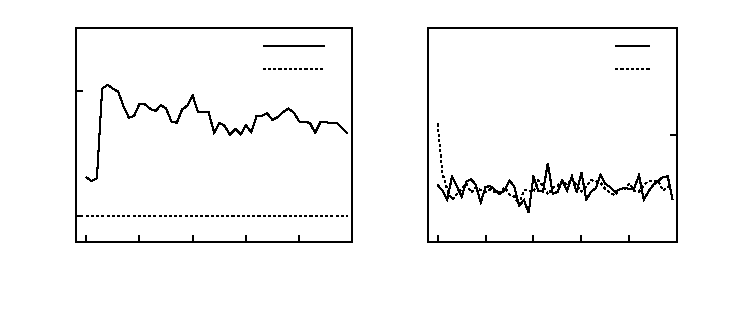
\includegraphics{R3}}%
    \gplfronttext
  \end{picture}%
\endgroup
}
\caption{Inventory and Backorder profile at $R3$}
\label{fig:esc:R3}
\end{figure}

Finally, in Table \ref{tab:esc:avgA}, we list the
average inventory at each node for products $A$ and $B$. Observe that
the average inventory at the nodes for the MPC policy is much closer
to the steady-state values, indicating that the MPC policy is
stabilizing. This example also illustrates the inherent robustness of
economic MPC as the controller was able to reject small variations in
demand around the nominal demand.

\begin{table}[h]
\caption{Average inventory for Product-A}
\label{tab:esc:avgA}
\begin{center}
\begin{tabular}{cccccccccc}\toprule
 &$M1$&$D1$&$D2$&$R1$&$R2$&$R3$&$R4$&$R5$\\ \midrule
MPC&58.01&17.48&12.36&0.34&5.43&7.71&0.26&3.44\\ 
Policy&82.91&10.70&6.02&0.011&1.39&3.21&0.23&5.47\\
\bottomrule 
\end{tabular}
\end{center}
\end{table}
\subsection{Scheduling model}
\label{sec:esc:multi:scheduling}
In the preceding sections, we did not consider the scheduling problem
at the manufacturing unit; instead, we approximated the production
delay using a constant production lead-time. In this section, we study
the economic MPC closed-loop performance for a supply chain which
includes a scheduling model for the manufacturing node.

We consider the same supply chain as in the previous section (Fig
\ref{fig:esc:lssc}), but with the following modification. The
manufacturing facility is assumed to have one unit $U$ which can
 make both products $A$ and $B$. The unit needs $3$ time units to make
$A$ via the task $\text{TA}$ and $2$ time units to make $B$ via the task
$\text{TB}$. In addition, there is changeover time of 1 unit whenever the
task is changed from $A$ to $B$ or vice-versa. 

Denote the set $\mathbf{I} = \set{\text{TA},\text{TB}}$,  $\text{PT}(i)$ as the
production lead time for each $i \in \mathbf{I}$ and $\text{CHT}(i,i')$ as
the changeover time between $i$ to $i'$. The scheduling constraints on
the manufacturing node can now be enforced by the following
inequalities (see \ref{sec:scheduling:example}):

\begin{alignat}{2}
&\sum_{i\in \mathbf{I}}\sum_{t' = t-\tau_i+1}^{t}W_{i,t'}+\sum_{i' \in
 \mathbf{I} \atop i' \neq i}\sum_{t'=t-\text{CHT}(i,i')+1}^{t}
Z_{i,i',t'} \leq 1 & \forall t \nonumber \\ 
&\sum_{t' = t-\tau_i+1}^{t} W_{i,t'} = Y_{i,t} & \forall t, \forall i
\in \mathbf{I} \nonumber\\
&X_{i,t} \geq Y_{i,t} & \forall t, \forall i \in \mathbf{I} \nonumber\\
&\sum_{i \in \mathbf{I}}X_{i,t} = 1 & \forall
t  \label{eq:esc:assign}\\ 
&Z_{i,i',t} \leq X_{i,t-1} &\forall t, \forall i \in \mathbf{I}, i' \in
\mathbf{I}, i' \neq i \nonumber\\
&Z_{i,i',t} \leq X_{i',t} &\forall t, \forall i \in \mathbf{I}, i' \in
\mathbf{I}, i'\neq i \nonumber \\
&Z_{i,i',t} \geq X_{i,t-1}+X_{i',t}-1 &\forall t, \forall i \in \mathbf{I}, i' \in
\mathbf{I}, i' \neq i \nonumber
\end{alignat}

To model the changeover time, we introduce three new binary variables $Z_{i,i',t},Y_{i,t}$ and
$X_{i,t}$. The binary variable $Z_{i,i',t}$ is 1 when a changeover is
effected from task $i$ to task $i'$ at time $t$. The binary variable
$Y_{i,t}$ is $1$ if the task $i$ was started during $[t-\tau_i,t]$. The
binary variable $X_{i,t}$ is 1 if the last task to be performed in the
unit before time $t$ was $i$.

In addition to these constraints, the batch-size is also controlled using
$W_{i,t}$ and the maximum and minimum batch-sizes. For the supply chain
studied, the maximum batch size was chosen to be $200$ for both the
products. The cost function corresponding to the new variables
included a cost to start a batch and a cost to effect a changeover
(see Table \ref{tab:esc:sched_prod}).

\begin{table*}
\caption{Production costs}
\label{tab:esc:sched_prod}
\begin{center}
\begin{tabular}{cc}\toprule
 &Cost \\ \midrule
Start a batch of TA & 10\\
Start a batch of TB & 6 \\
Changeover from TA to TB & 10\\
Changeover from TB to TA & 5\\
\bottomrule 
\end{tabular}
\end{center}
\end{table*}


Following the procedure outlined in
Chapter \ref{chap:scheduling}, we can write the supply
chain dynamics with the binary variables in the state space format
\eqref{eq:esc:model}. We denote the state space model of the
manufacturer scheduling problem as

\begin{equation}
x_M^+ = A_Mx_M + B_Mu_M + B_{d,M}u_{-M}
\end{equation}

in which $u_{-M}$ are the inputs of the other nodes in the supply chain, that is, the
shipping and ordering among $(D1,D2,R1 - R5)$ as well as the orders
placed by them to $M1$. The input $u_M$ consists of shipments sent by
the manufacturer to  the other nodes, and the binary decisions given
in \eqref{eq:esc:assign}. 

Therefore, we can easily write the whole supply chain dynamics model in
the state space form \eqref{eq:esc:model}. We only note that the
inputs now include the binary choices at the manufacturer and the
constraint set, instead of being just $x \in \mathbb{X}, u \in \mathbb{U}$,
becomes
\begin{gather}
\label{eq:esc:constraints}
 x \in \mathbb{X}, u \in \mathbb{U} \\
 \underline{b} \leq E_x x(t) + E_u u(t) \leq \overline{b}
\end{gather}

with the second inequality representing the assignment constraint
\eqref{eq:esc:assign} in the state space form.


We now define the periodic optimization problem that is used to find a
sub-optimal infinite horizon schedule and shipping/ordering policies
in response to the nominal demand given in Table \ref{tab:esc:nomdem}. In
the previous section, we found the steady-state shipping and ordering
so that the supply chain returns to the same state at the next
sampling instance. In this section, we find a periodic policy 
so that after $N_{p}$ sampling periods, the supply chain returns to the starting
state. The interpretation is that, if we observe the  nominal demands over
an infinite horizon, then we can remain feasible with the periodic
policy (by repeating it infinitely).
The optimization problem solved is \footnote{Note that we are solving
  a purely economic problem}:

\begin{alignat}{2}
\label{eq:esc:Pp}
\mathbb{P}_p:& \min_{\bu,x(0)}{\sum_{i=0}^{N_p-1}\ell_E(x(i),u(i),d_s(i))}& \nonumber \\
&\text{s.t.~} x(i+1) = Ax(i) + Bu(i)+B_dd_s(i),&i = \set{0,1,\ldots,N_p-1} \\
& \text{Constraints}\eqref{eq:esc:constraints}&i = \set{0,1,\ldots,N_p-1} \nonumber\\
& x(0) = x(N_p)& \nonumber\\
\end{alignat}
in which $N_p$ is the period.  We denote the solution to
\eqref{eq:esc:Pp} by $(\mathbf{u}_p^0,x(0)_p^0)$,
The solution to \eqref{eq:esc:Pp} gives us the periodic state-profile
\begin{equation}
\label{eq:esc:Xperiodic}
\mathbb{X}_p =  \set {x^0_p(0),x(1;x^0_p(0),\bu_p^0,\bd_s),\ldots,x(N_p;x^0_p(0),\bu_p^0,\bd_s) }
\end{equation}

In Figure \ref{fig:esc:gantt_ss}, we show the Gantt chart for the periodic
schedule with $N_p = 24$.

\begin{figure}
\centering
\scriptsize
\centering
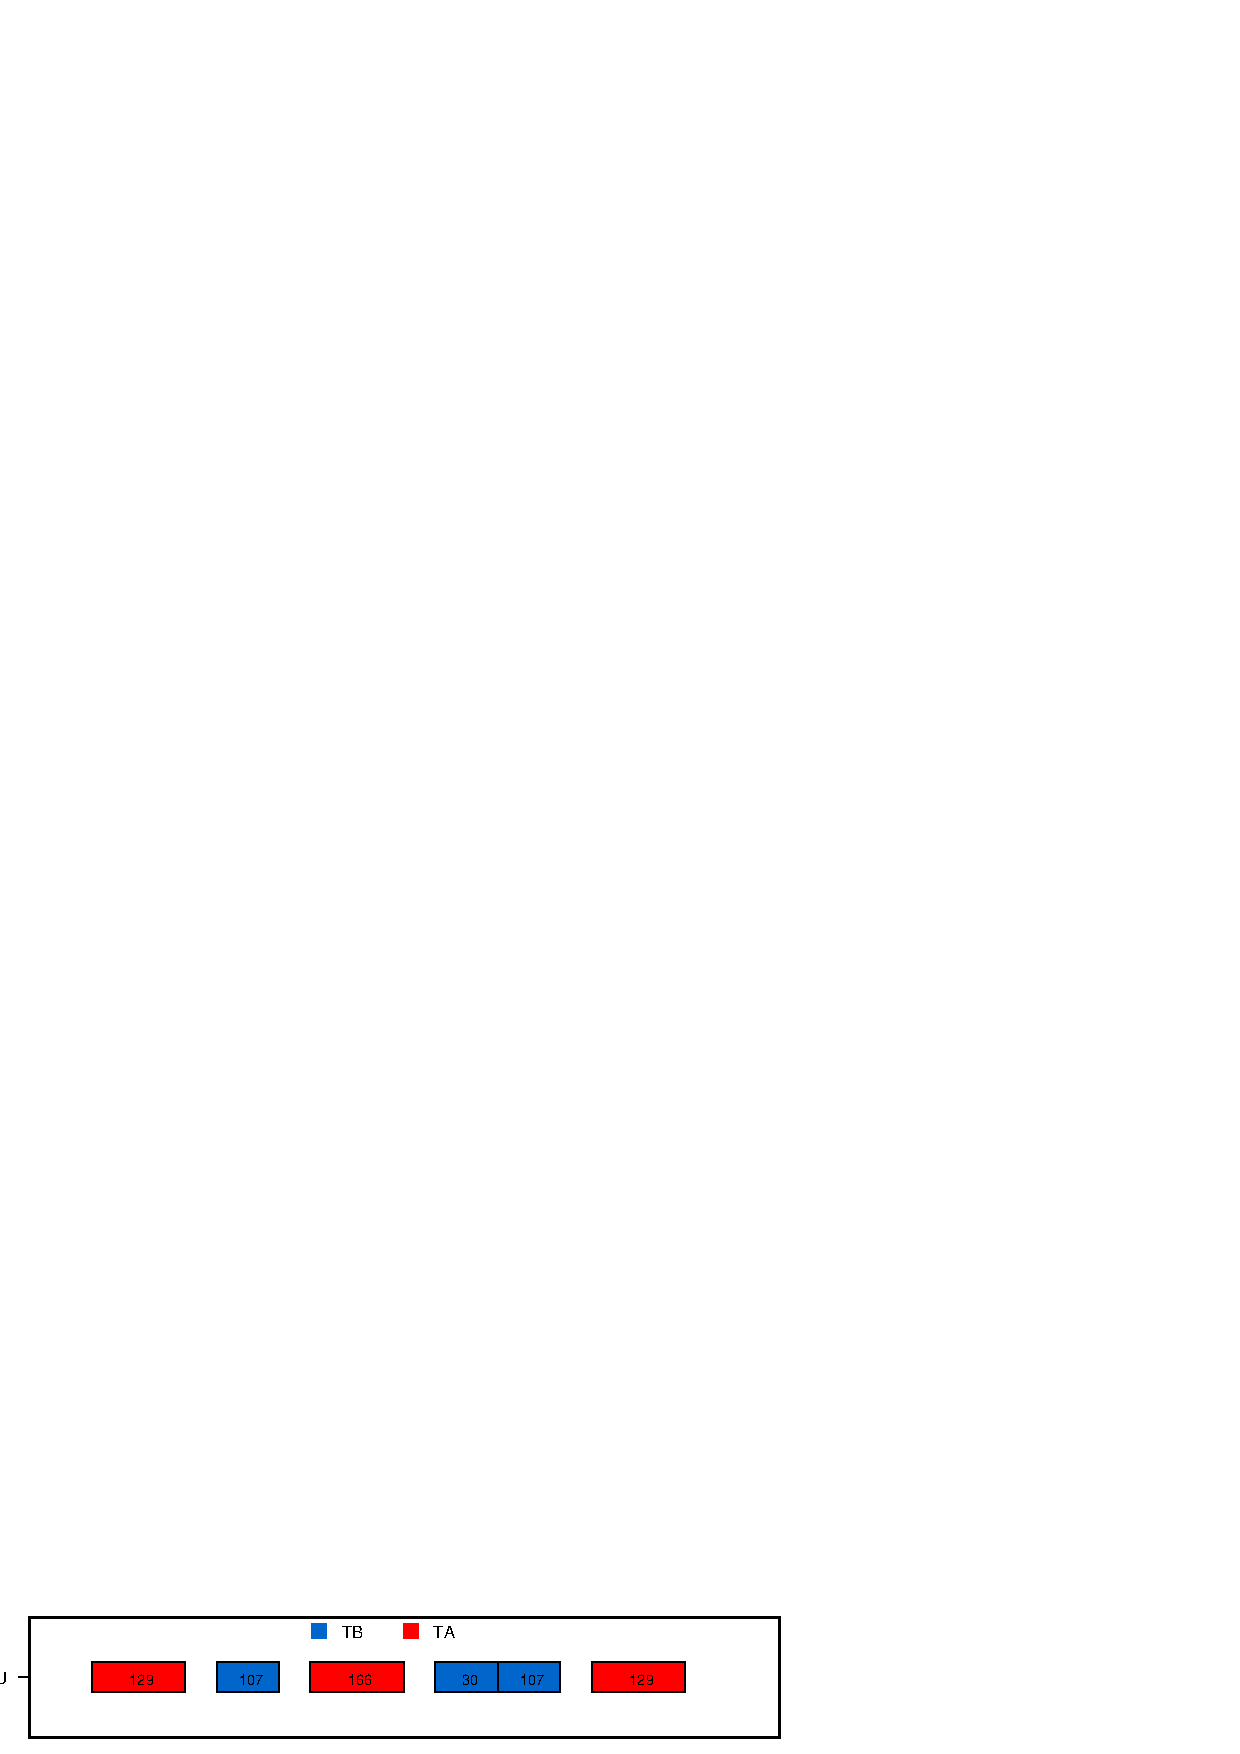
\includegraphics{esc/SS_gantt.pdf}
\caption{Periodic production schedule to respond to nominal demands}
\label{fig:esc:gantt_ss}

\label{fig:esc:ganttTNT1}
\begin{center}
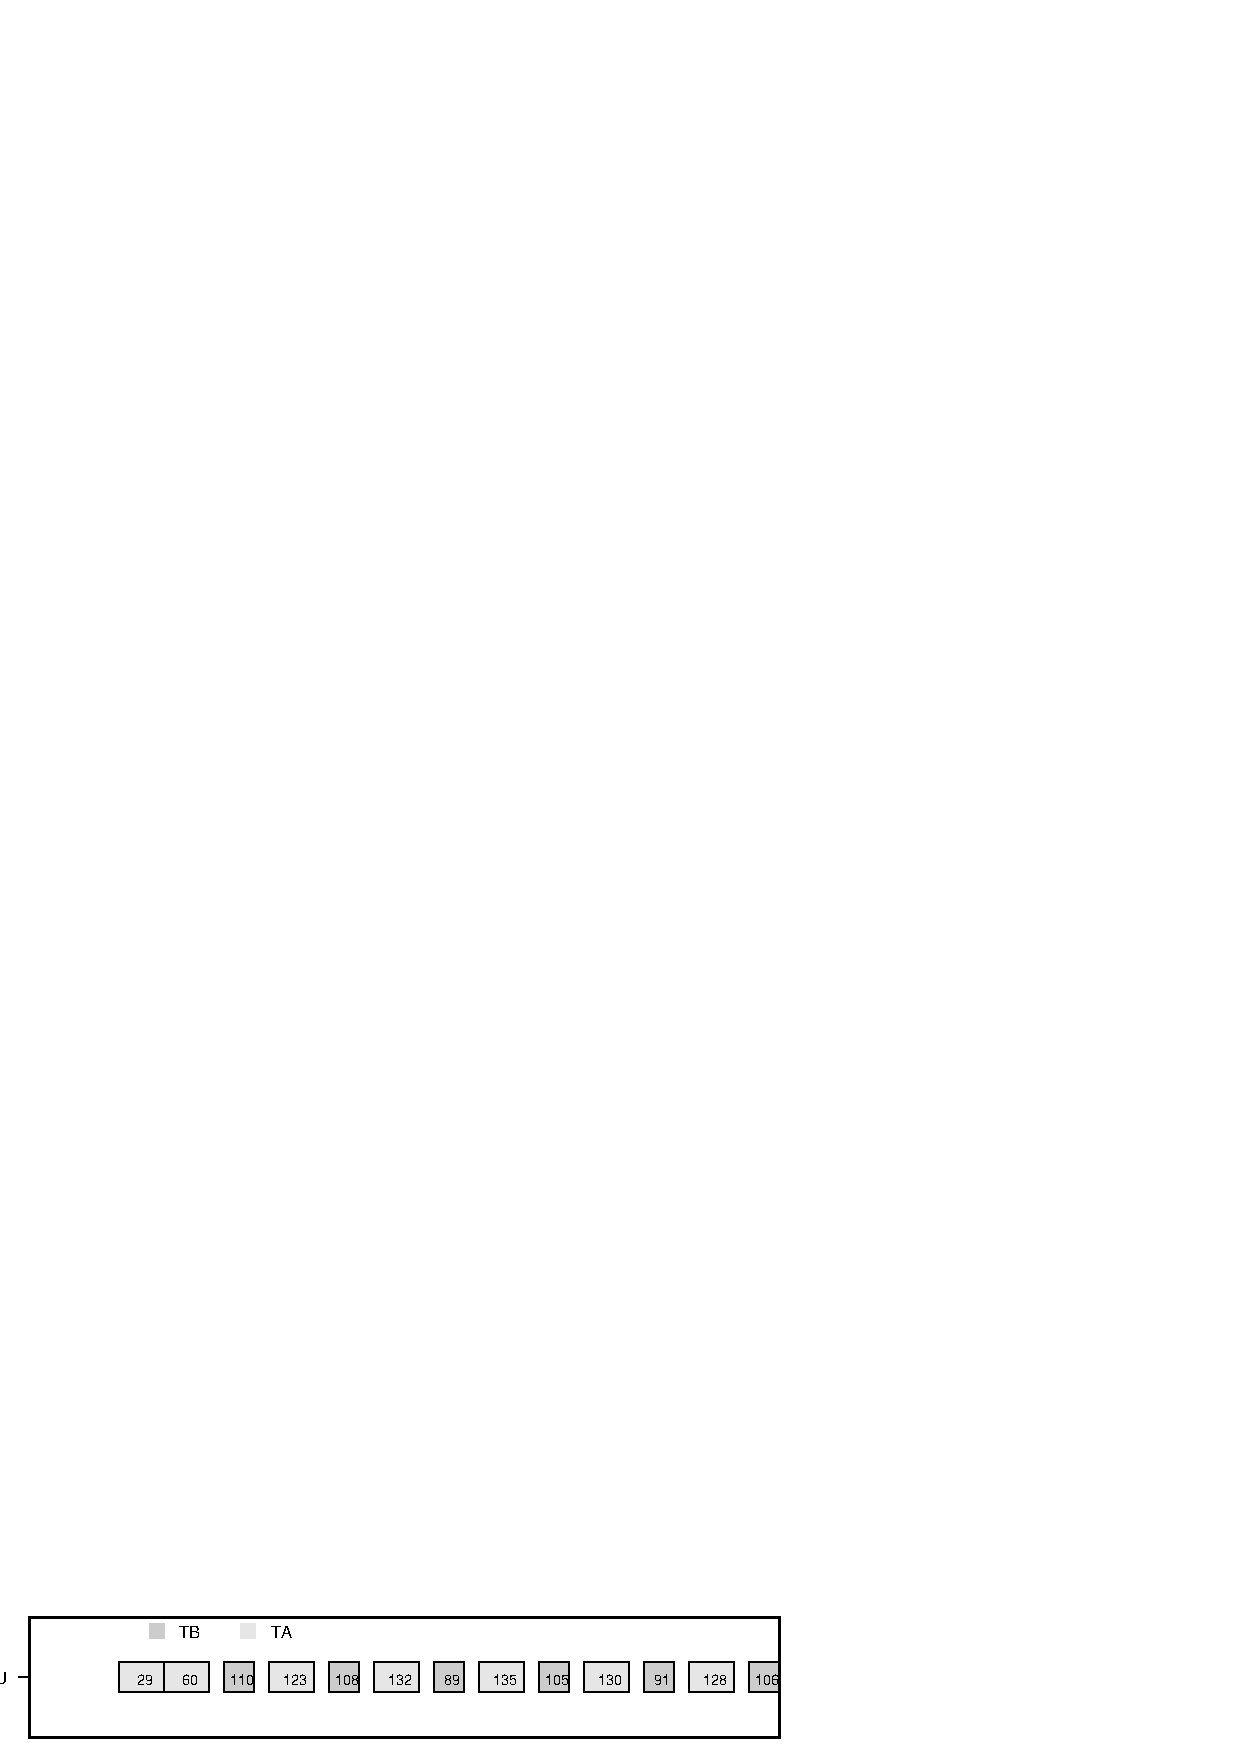
\includegraphics{esc/NTS_gantt.pdf}
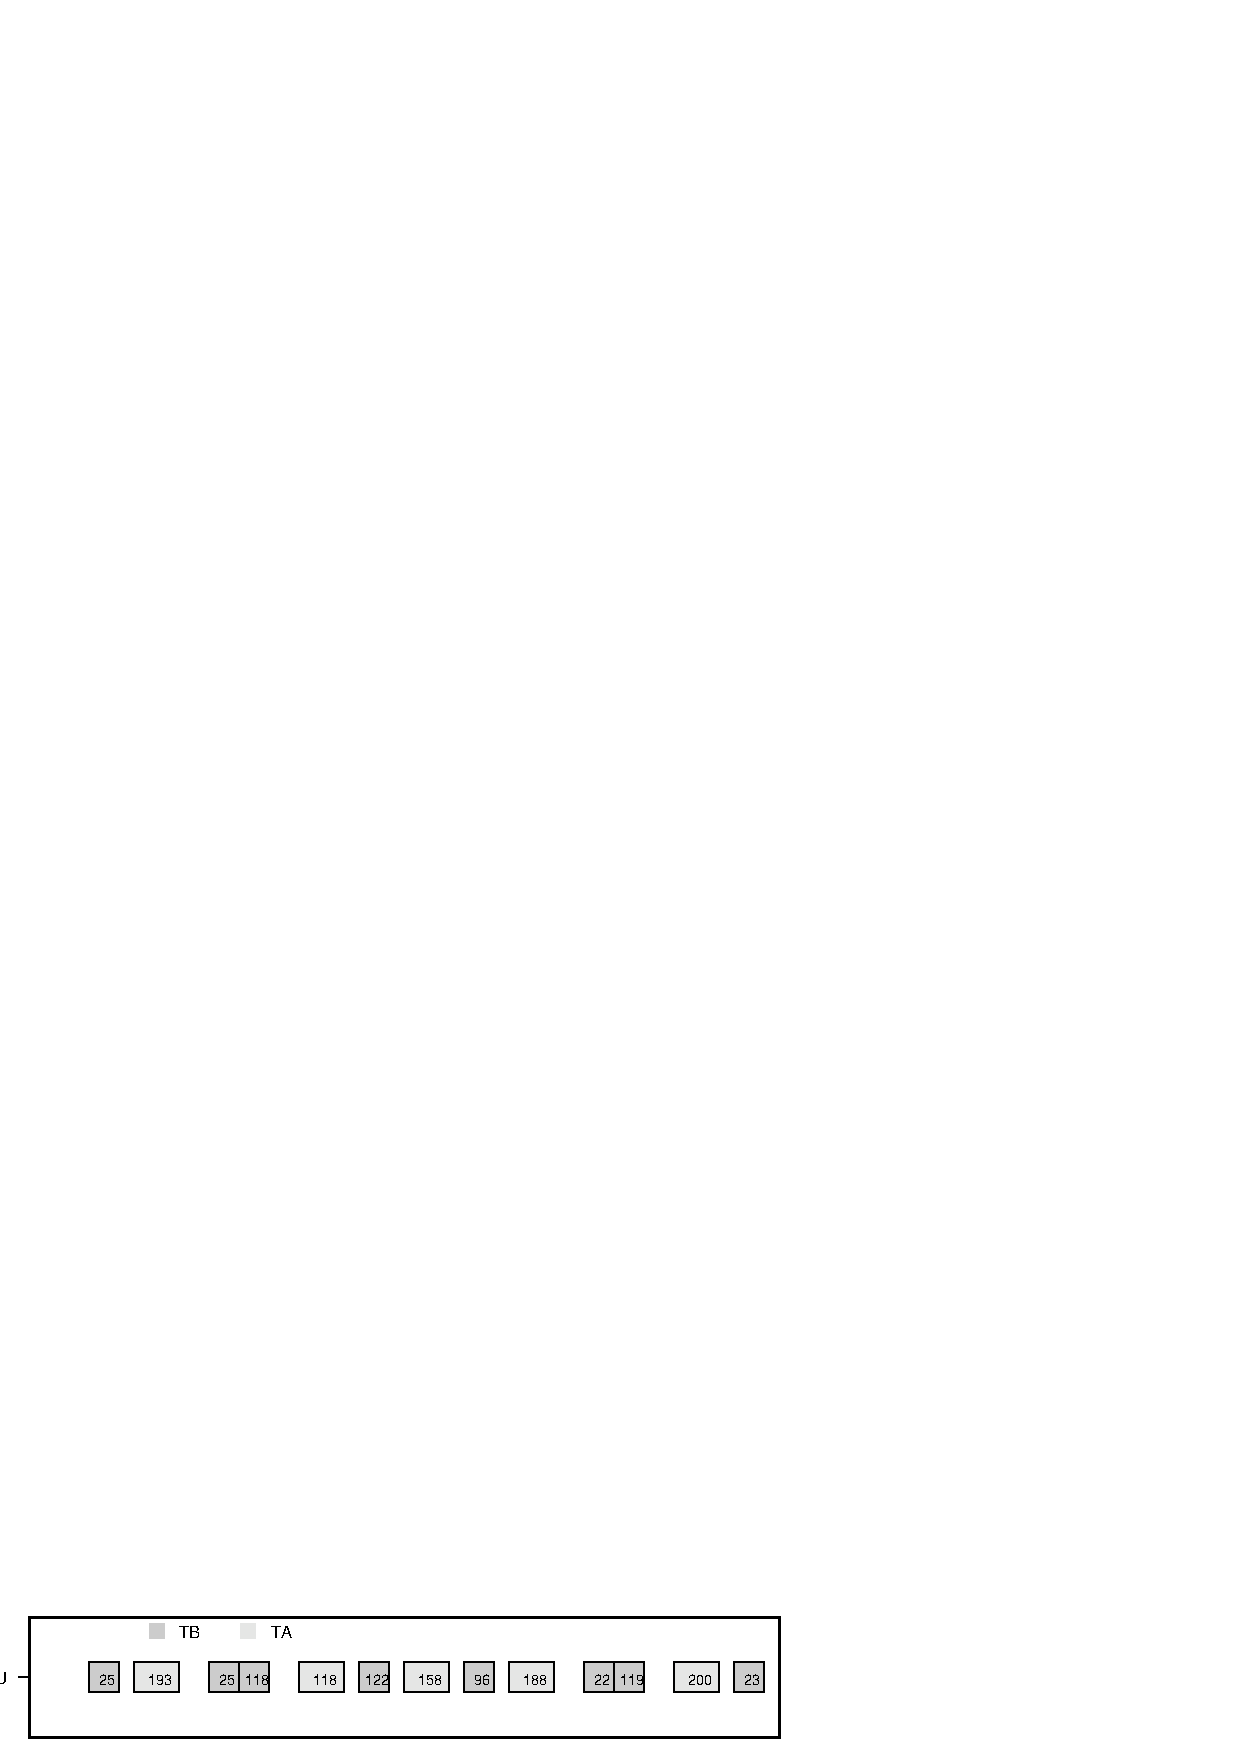
\includegraphics{esc/TS_gantt.pdf}
\caption{Production schedule for the MPC without terminal constraints that optimized
  \eqref{eq:esc:PbNT} (Top) compared with production schedule for the MPC
  with terminal constraints that optimized \eqref{eq:esc:PbT}. Note how larger batches are made for
  the problem with terminal constraints}
\end{center}
\end{figure}

\begin{figure}
\centering
\scriptsize
\resizebox{1\textwidth}{!}{% GNUPLOT: LaTeX picture with Postscript
\begingroup
  \makeatletter
  \providecommand\color[2][]{%
    \GenericError{(gnuplot) \space\space\space\@spaces}{%
      Package color not loaded in conjunction with
      terminal option `colourtext'%
    }{See the gnuplot documentation for explanation.%
    }{Either use 'blacktext' in gnuplot or load the package
      color.sty in LaTeX.}%
    \renewcommand\color[2][]{}%
  }%
  \providecommand\includegraphics[2][]{%
    \GenericError{(gnuplot) \space\space\space\@spaces}{%
      Package graphicx or graphics not loaded%
    }{See the gnuplot documentation for explanation.%
    }{The gnuplot epslatex terminal needs graphicx.sty or graphics.sty.}%
    \renewcommand\includegraphics[2][]{}%
  }%
  \providecommand\rotatebox[2]{#2}%
  \@ifundefined{ifGPcolor}{%
    \newif\ifGPcolor
    \GPcolortrue
  }{}%
  \@ifundefined{ifGPblacktext}{%
    \newif\ifGPblacktext
    \GPblacktexttrue
  }{}%
  % define a \g@addto@macro without @ in the name:
  \let\gplgaddtomacro\g@addto@macro
  % define empty templates for all commands taking text:
  \gdef\gplbacktext{}%
  \gdef\gplfronttext{}%
  \makeatother
  \ifGPblacktext
    % no textcolor at all
    \def\colorrgb#1{}%
    \def\colorgray#1{}%
  \else
    % gray or color?
    \ifGPcolor
      \def\colorrgb#1{\color[rgb]{#1}}%
      \def\colorgray#1{\color[gray]{#1}}%
      \expandafter\def\csname LTw\endcsname{\color{white}}%
      \expandafter\def\csname LTb\endcsname{\color{black}}%
      \expandafter\def\csname LTa\endcsname{\color{black}}%
      \expandafter\def\csname LT0\endcsname{\color[rgb]{1,0,0}}%
      \expandafter\def\csname LT1\endcsname{\color[rgb]{0,1,0}}%
      \expandafter\def\csname LT2\endcsname{\color[rgb]{0,0,1}}%
      \expandafter\def\csname LT3\endcsname{\color[rgb]{1,0,1}}%
      \expandafter\def\csname LT4\endcsname{\color[rgb]{0,1,1}}%
      \expandafter\def\csname LT5\endcsname{\color[rgb]{1,1,0}}%
      \expandafter\def\csname LT6\endcsname{\color[rgb]{0,0,0}}%
      \expandafter\def\csname LT7\endcsname{\color[rgb]{1,0.3,0}}%
      \expandafter\def\csname LT8\endcsname{\color[rgb]{0.5,0.5,0.5}}%
    \else
      % gray
      \def\colorrgb#1{\color{black}}%
      \def\colorgray#1{\color[gray]{#1}}%
      \expandafter\def\csname LTw\endcsname{\color{white}}%
      \expandafter\def\csname LTb\endcsname{\color{black}}%
      \expandafter\def\csname LTa\endcsname{\color{black}}%
      \expandafter\def\csname LT0\endcsname{\color{black}}%
      \expandafter\def\csname LT1\endcsname{\color{black}}%
      \expandafter\def\csname LT2\endcsname{\color{black}}%
      \expandafter\def\csname LT3\endcsname{\color{black}}%
      \expandafter\def\csname LT4\endcsname{\color{black}}%
      \expandafter\def\csname LT5\endcsname{\color{black}}%
      \expandafter\def\csname LT6\endcsname{\color{black}}%
      \expandafter\def\csname LT7\endcsname{\color{black}}%
      \expandafter\def\csname LT8\endcsname{\color{black}}%
    \fi
  \fi
  \setlength{\unitlength}{0.0500bp}%
  \begin{picture}(7200.00,3024.00)%
    \gplgaddtomacro\gplbacktext{%
      \csname LTb\endcsname%
      \put(946,714){\makebox(0,0)[r]{\strut{} 0}}%
      \put(946,919){\makebox(0,0)[r]{\strut{} 10}}%
      \put(946,1123){\makebox(0,0)[r]{\strut{} 20}}%
      \put(946,1328){\makebox(0,0)[r]{\strut{} 30}}%
      \put(946,1532){\makebox(0,0)[r]{\strut{} 40}}%
      \put(946,1737){\makebox(0,0)[r]{\strut{} 50}}%
      \put(946,1941){\makebox(0,0)[r]{\strut{} 60}}%
      \put(946,2146){\makebox(0,0)[r]{\strut{} 70}}%
      \put(946,2350){\makebox(0,0)[r]{\strut{} 80}}%
      \put(946,2555){\makebox(0,0)[r]{\strut{} 90}}%
      \put(946,2759){\makebox(0,0)[r]{\strut{} 100}}%
      \put(1078,484){\makebox(0,0){\strut{} 0}}%
      \put(2223,484){\makebox(0,0){\strut{} 10}}%
      \put(3368,484){\makebox(0,0){\strut{} 20}}%
      \put(4513,484){\makebox(0,0){\strut{} 30}}%
      \put(5658,484){\makebox(0,0){\strut{} 40}}%
      \put(6803,484){\makebox(0,0){\strut{} 50}}%
      \put(176,1731){\rotatebox{-270}{\makebox(0,0){\strut{}Backorder -Retailer}}}%
      \put(3940,154){\makebox(0,0){\strut{}Time}}%
    }%
    \gplgaddtomacro\gplfronttext{%
      \csname LTb\endcsname%
      \put(5816,2586){\makebox(0,0)[r]{\strut{}Without terminal constraint}}%
      \csname LTb\endcsname%
      \put(5816,2366){\makebox(0,0)[r]{\strut{}With terminal constraint}}%
    }%
    \gplbacktext
    \put(0,0){\includegraphics{BOprofile}}%
    \gplfronttext
  \end{picture}%
\endgroup
}
\caption{Combined backorder at all the retailer nodes}
\label{fig:esc:BOTNT}
\end{figure}

\subsubsection{Dynamic Response}
In this section, we show the dynamic response to a stochastic demand
signal.

We first consider the closed-loop solution, in which, at each sampling
time optimization problem \eqref{eq:esc:PbNT} is solved, and compare it
with the closed-loop solution in which the optimization problem
\eqref{eq:esc:PbT} is solved. In \eqref{eq:esc:PbT}, we force the final state
to lie on the periodic profile $\mathbb{X}_p$. Hence, at the end of
the planning horizon $N$, the supply-chain is at a state from which it
can respond to the nominal demand. In contrast, for the optimization
problem \eqref{eq:esc:PbNT}, the terminal state is chosen without
considering future demands that arrive after the planning horizon
$N$. Therefore, the solutions to \eqref{eq:esc:PbNT} have (i) fewer
production and (ii) lesser inventory at nodes. This leads to
increasing backorders when new demands are observed at the next
sampling time. In Figure \ref{fig:esc:BOTNT}, we compare the backorders
observed in the closed-loop when the MPC optimizer solved
\eqref{eq:esc:PbNT} and \eqref{eq:esc:PbT}. In Figure \ref{fig:esc:ganttTNT1}, we
show the Gantt chart for the implemented schedule by the two MPCs. The
planning horizon used was $N = 12$. Note that, under the presence of
persistent disturbance (that is different from the nominal
disturbance), the MPC design has to be robust
\citep[Ch 3.]{rawlings:mayne:2009}. In this example, we have not
designed robust-MPC but instead the results show the inherent-robustness of
nominal MPC to reject small deviations from the nominal
demand. 
 
\begin{alignat}{2}
\label{eq:esc:PbNT}
\mathbb{P}_N(x):& \min_{\bu}
{\sum_{i=0}^{N-1}\ell_E(x(j),u(j),d(j))}& \nonumber \\
&\text{s.t.~} x(j+1) = Ax(j) + Bu(j)+B_dd_s(j),&j = \set{0,1,\ldots,N-1}\\\
& \text{Constraints}\eqref{eq:esc:constraints}&j = \set{0,1,\ldots,N-1} \nonumber\\
& x(0) = x \nonumber\\
\end{alignat}

\begin{alignat}{2}
\label{eq:esc:PbT}
\mathbb{P}_N(x):& \min_{\bu}
{\sum_{i=0}^{N-1}\ell_E(x(j),u(j),d(j))}& \nonumber \\
&\text{s.t.~} x(j+1) = Ax(j) + Bu(j)+B_dd_s(j),&j = \set{0,1,\ldots,N-1}\\\
& \text{Constraints}\eqref{eq:esc:constraints}&j = \set{0,1,\ldots,N-1} \nonumber\\
& x(0) = x \nonumber\\
& x(N) \in \mathbb{X}_P
\end{alignat}







